\appendix
\newcounter{finalframe}
\setcounter{finalframe}{\value{framenumber}}


\subsubsection{Advection vs. Diffusion Sensitivity GDSM Results}

In the parametric sensitivity analysis discussed in section
\ref{sec:AdvVelDiffCoeff}, it was shown that for isotopes of interest, higher
advective velocity and higher diffusivity lead to higher peak annual doses. 
However, the relationship between diffusivity and advective
velocity adds depth to the notion of a boundary between diffusive and advective
regimes.

The highly soluble and non-sorbing elements, $I$ and $Cl$ 
were expected to exhibit behavior that is highly sensitive 
to advection in the system in the advective regime but less sensitive to 
advection in the diffusive regime.  

In Figures \ref{fig:VAdvVelI129}, \ref{fig:VAdvVelI129VAdvVel}, 
\ref{fig:VAdvVelCl36}, and \ref{fig:VAdvVelCl36VAdvVel} , $^{129}I$ and 
$^{36}Cl$ are more sensitive to vertical advective velocity for lower vertical 
advective velocities. This demonstrates that for vertical advective velocities 
$6.31\times10^{-6}$ m/yr and above, lower reference diffusivities are 
ineffective at attenuating the mean of the peak doses for soluble, non-sorbing 
elements. 

\begin{figure}[htp!]
\begin{minipage}[b]{0.45\linewidth}
\centering
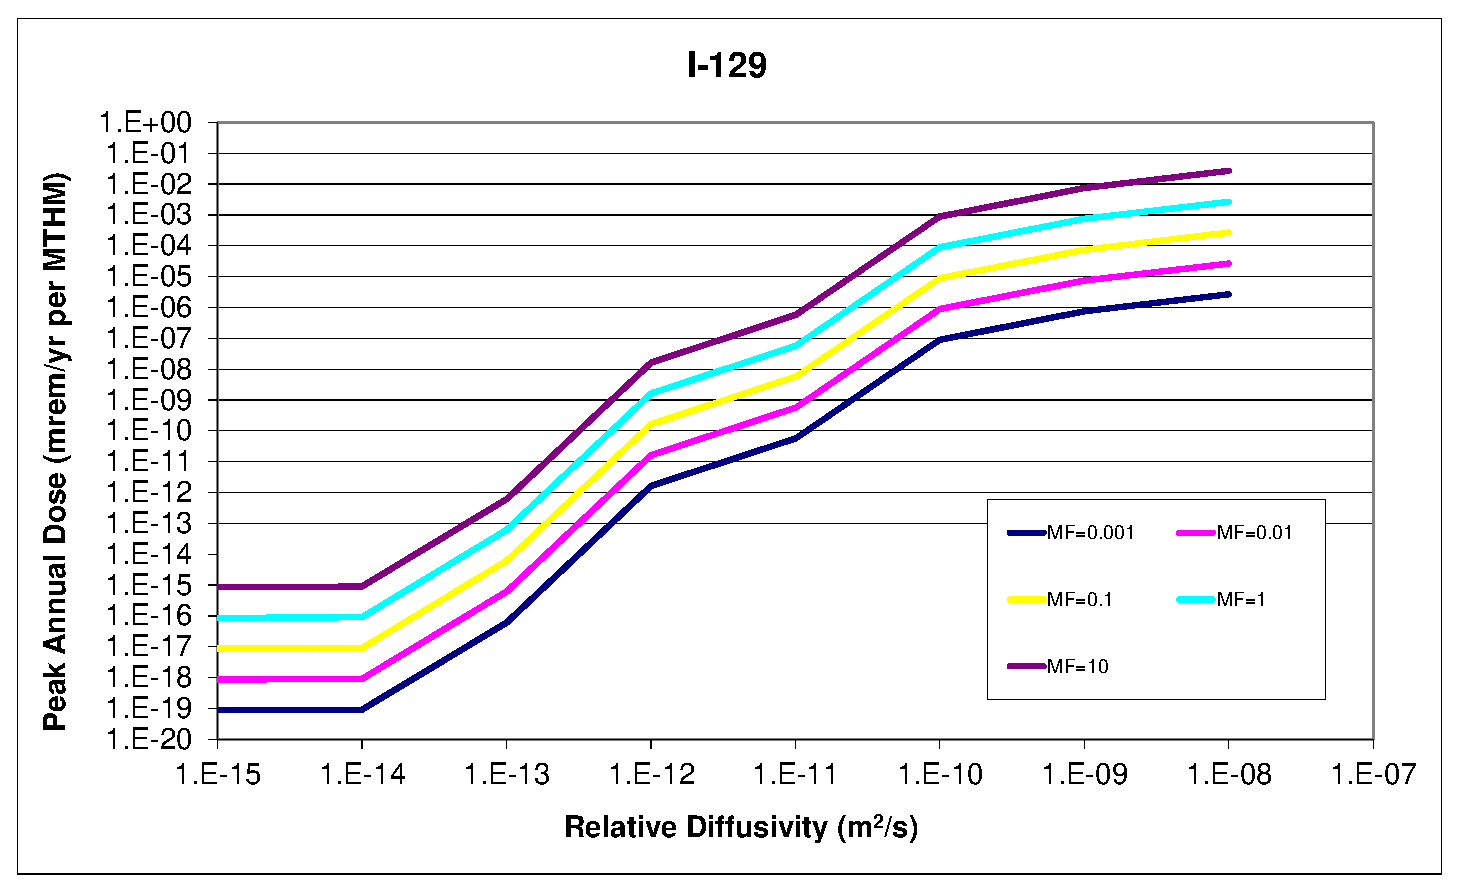
\includegraphics[width=\linewidth]{./chapters/nuclide_sensitivity/clay/AdvVelAndDiffCoeffEBSFail/I-129.eps}
\caption{$^{129}I$ reference diffusivity sensitivity.}
\label{fig:VAdvVelI129}

\end{minipage}
\hspace{0.05\linewidth}
\begin{minipage}[b]{0.45\linewidth}

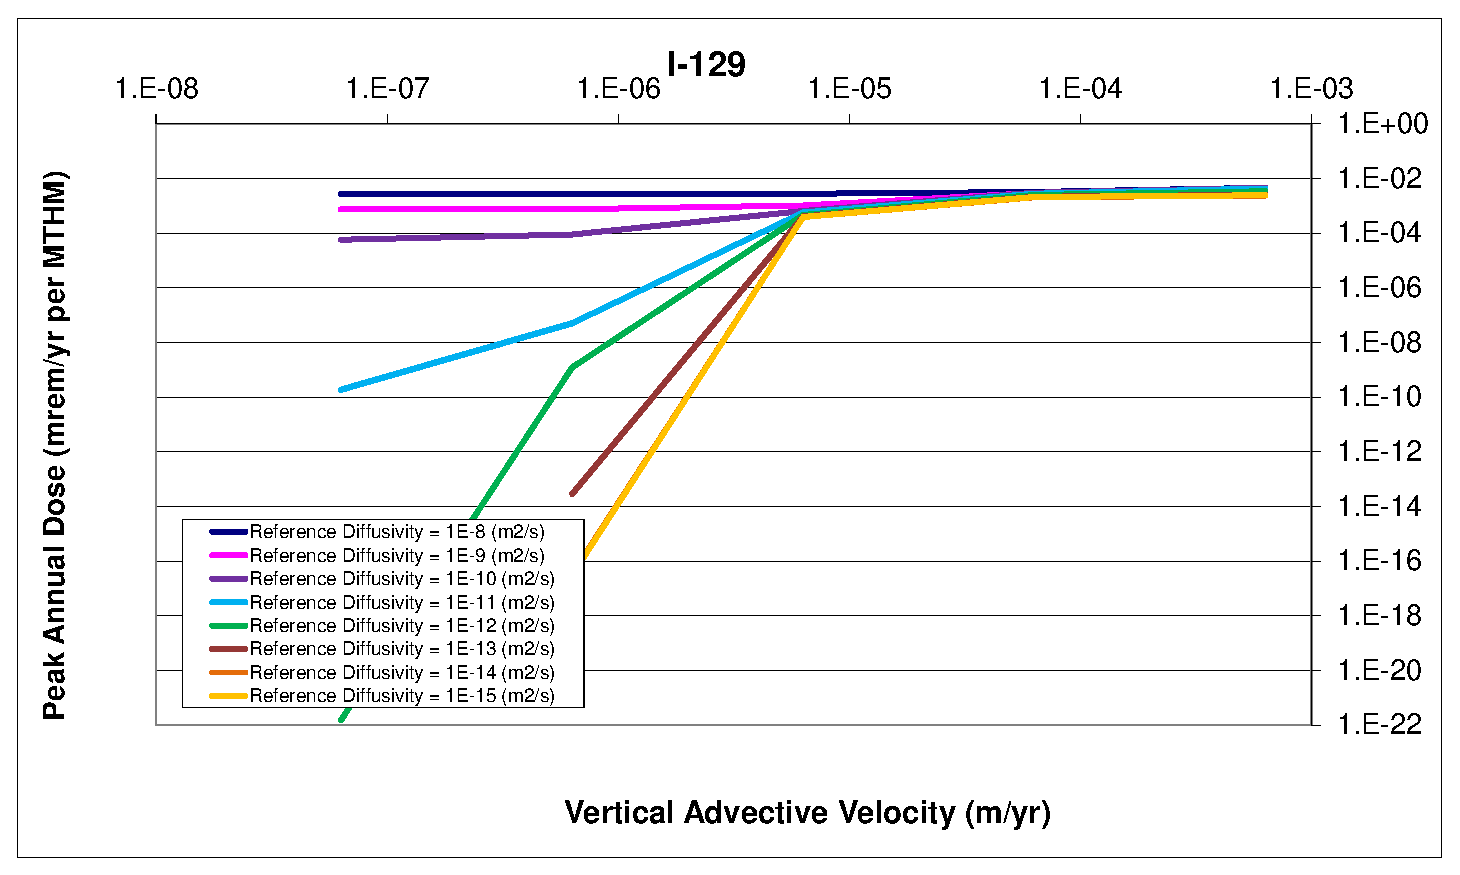
\includegraphics[width=\linewidth]{./chapters/nuclide_sensitivity/clay/AdvVelAndDiffCoeffEBSFail/I-129-VAdvVel.eps}
\caption{$^{129}I$ vertical advective velocity sensitivity.}
\label{fig:VAdvVelI129VAdvVel}

\end{minipage}
\end{figure}

\begin{figure}[htp!]
\begin{minipage}[b]{0.45\linewidth}

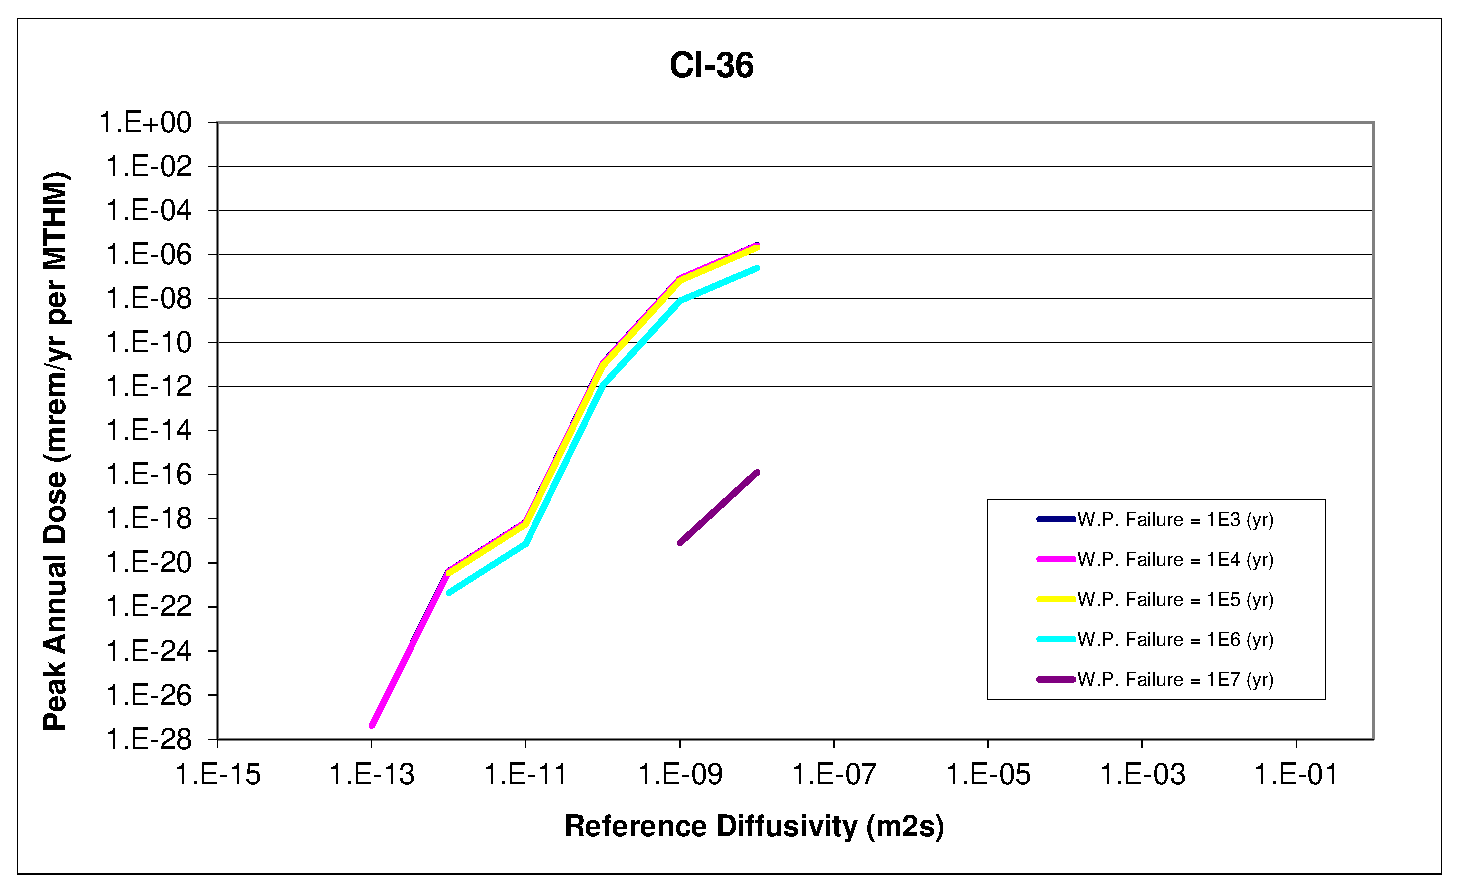
\includegraphics[width=\textwidth]{./chapters/nuclide_sensitivity/clay/AdvVelAndDiffCoeffEBSFail/Cl-36.eps}
\caption{$^{36}Cl$ reference diffusivity sensitivity.}
\label{fig:VAdvVelCl36}

\end{minipage}
\hspace{0.05\linewidth}
\begin{minipage}[b]{0.45\linewidth}

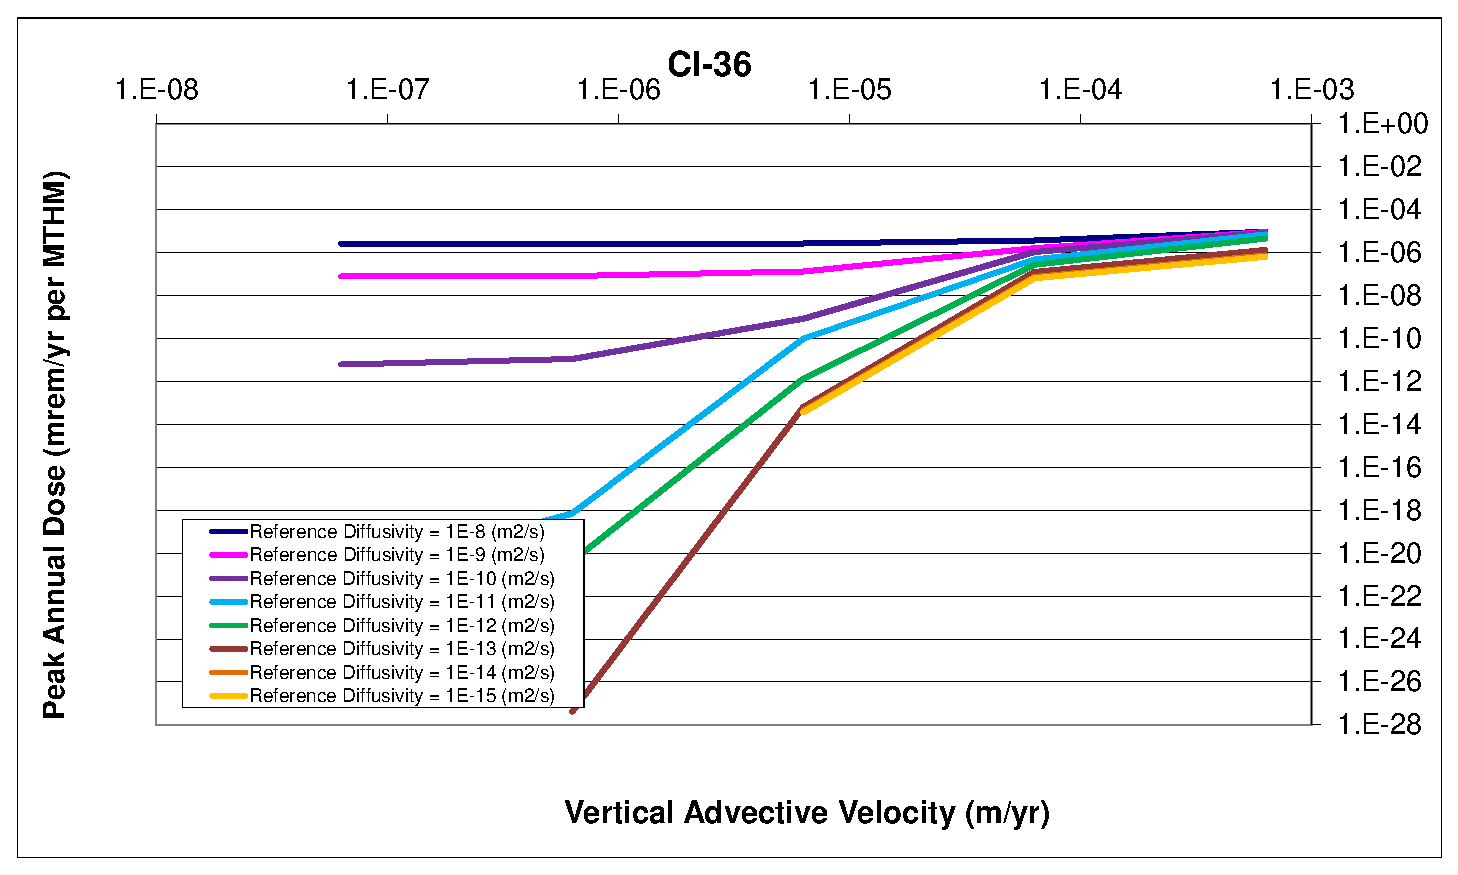
\includegraphics[width=\textwidth]{./chapters/nuclide_sensitivity/clay/AdvVelAndDiffCoeffEBSFail/Cl-36-VAdvVel.eps}
\caption{$^{36}Cl$ vertical advective velocity sensitivity.}
\label{fig:VAdvVelCl36VAdvVel}
\end{minipage}
\end{figure}

The solubility limited and sorbing elements, $Tc$ and $Np$, in Figures 
\ref{fig:VAdvVelTc99}, \ref{fig:VAdvVelTc99VAdvVel}, \ref{fig:VAdvVelNp237}, and 
\ref{fig:VAdvVelNp237VAdvVel} show a very weak influence on peak annual dose 
rate for low reference diffusivities, but show a direct proportionality between 
dose and reference diffusivity above a threshold. For $^{99}Tc$, for example, 
that threshold occurs at $1\times10^{-11}$ m$^2$/s. 


Dose contribution from $^{99}Tc$ has a proportional 
relationship with vertical advective velocity above a regime threshold at 
$6.31\times10^{-5}$ m/yr, above which the system exhibits sensitivity to 
advection. 

%There is an interesting feature in which $^{99}Tc$ 
%exhibits a decrease in peak annual dose for an increase in reference diffusivity 
%for the very high ($6.31\times10^{-4}$) vertcial advective velocity case. %WHY? 

\begin{figure}[htp!]
\begin{minipage}[b]{0.45\linewidth}
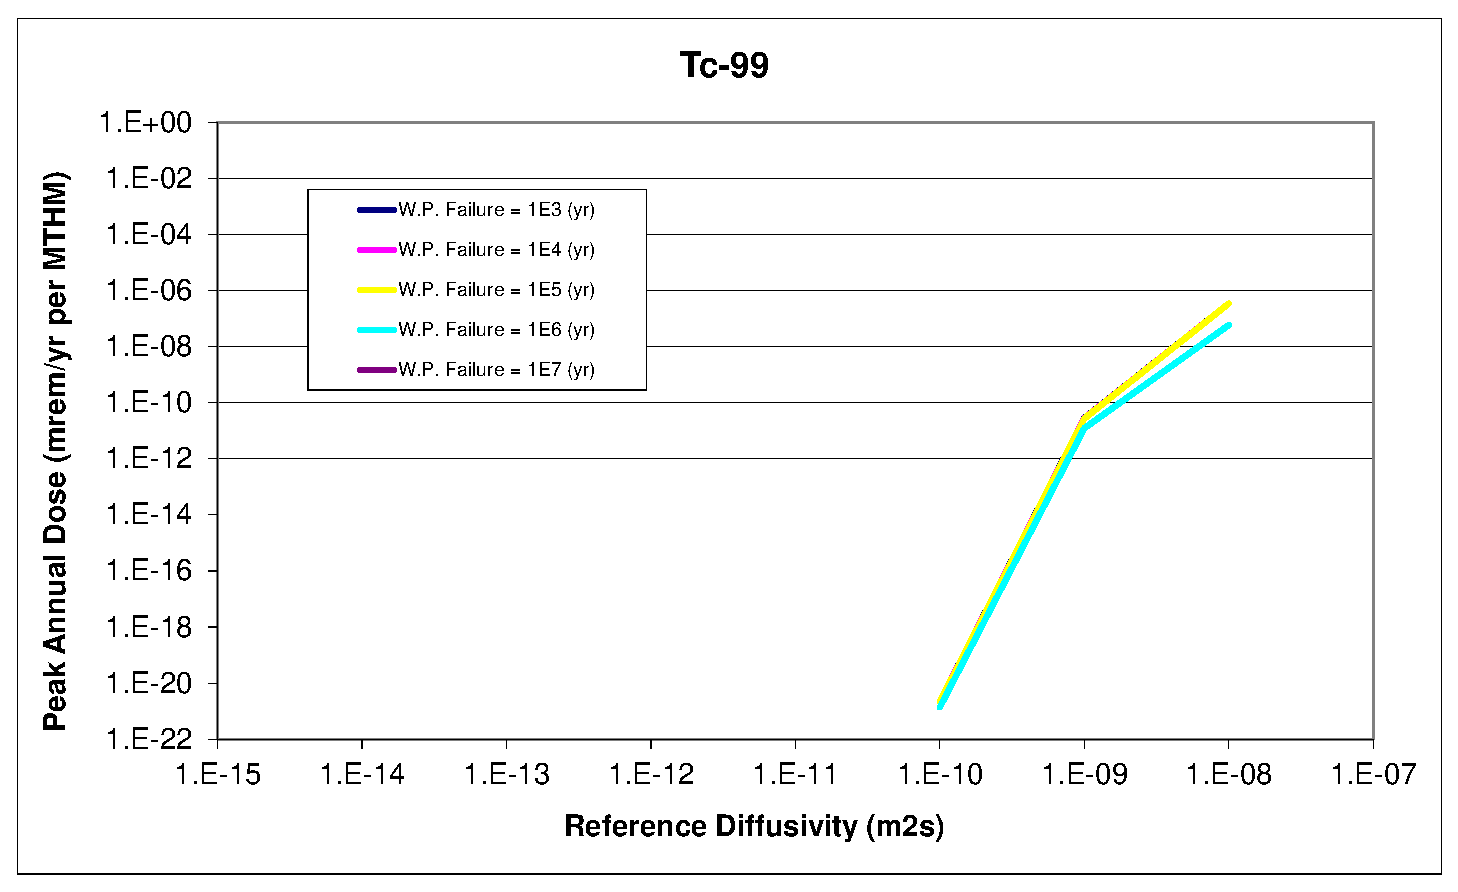
\includegraphics[width=\linewidth]{./chapters/nuclide_sensitivity/clay/AdvVelAndDiffCoeffEBSFail/Tc-99.eps}
\caption{$^{99}Tc$ reference diffusivity sensitivity.}
\label{fig:VAdvVelTc99}

\end{minipage}
\hspace{0.05\linewidth}
\begin{minipage}[b]{0.45\linewidth}

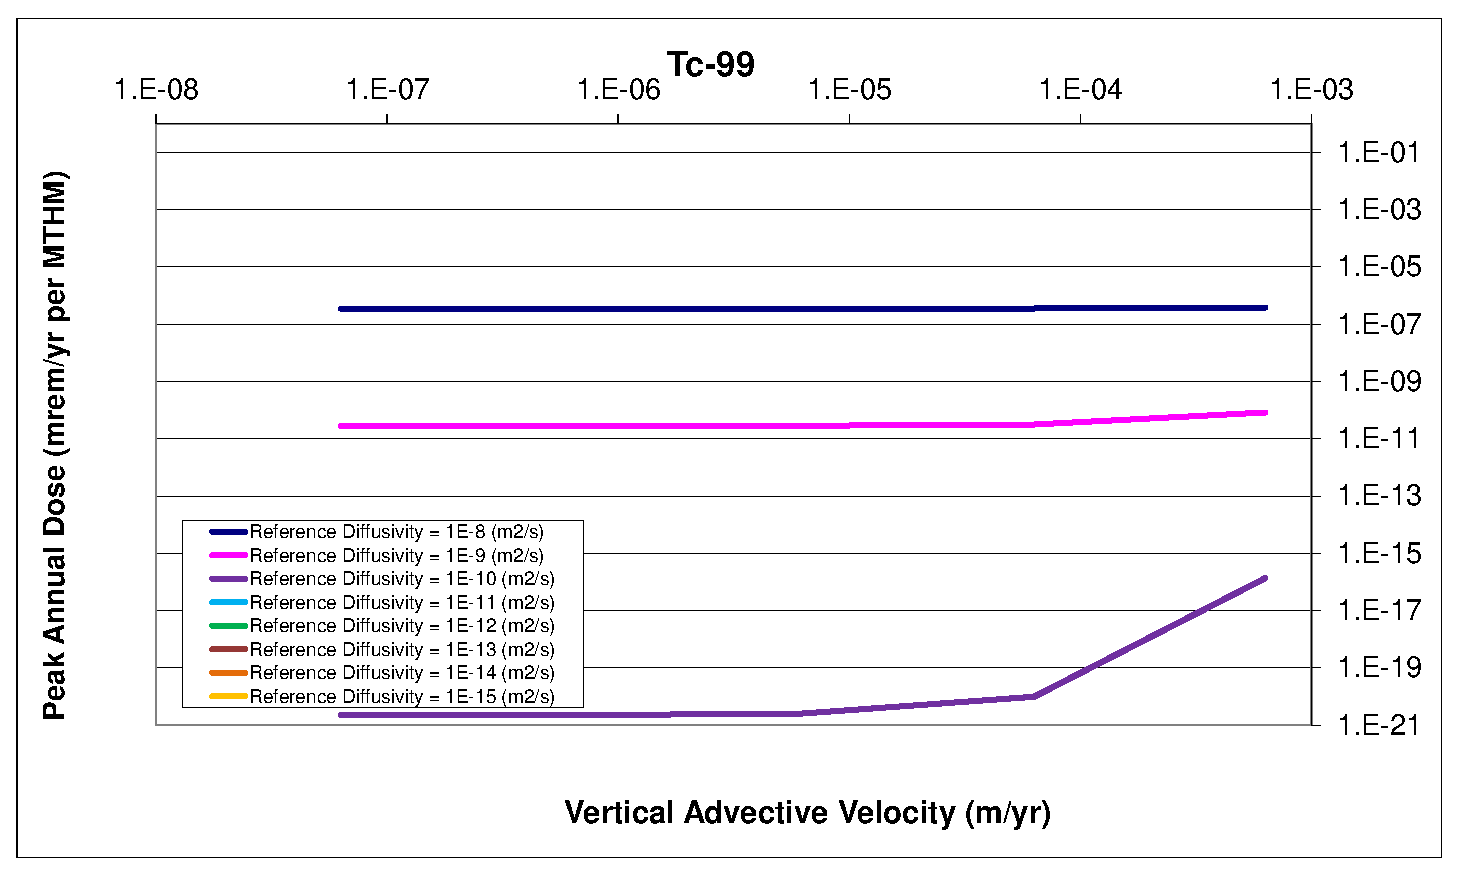
\includegraphics[width=\linewidth]{./chapters/nuclide_sensitivity/clay/AdvVelAndDiffCoeffEBSFail/Tc-99-VAdvVel.eps}
\caption{$^{99}Tc$ vertical advective velocity sensitivity.}
\label{fig:VAdvVelTc99VAdvVel}

\end{minipage}
\end{figure}

\begin{figure}[htp!]
\begin{minipage}[b]{0.45\linewidth}
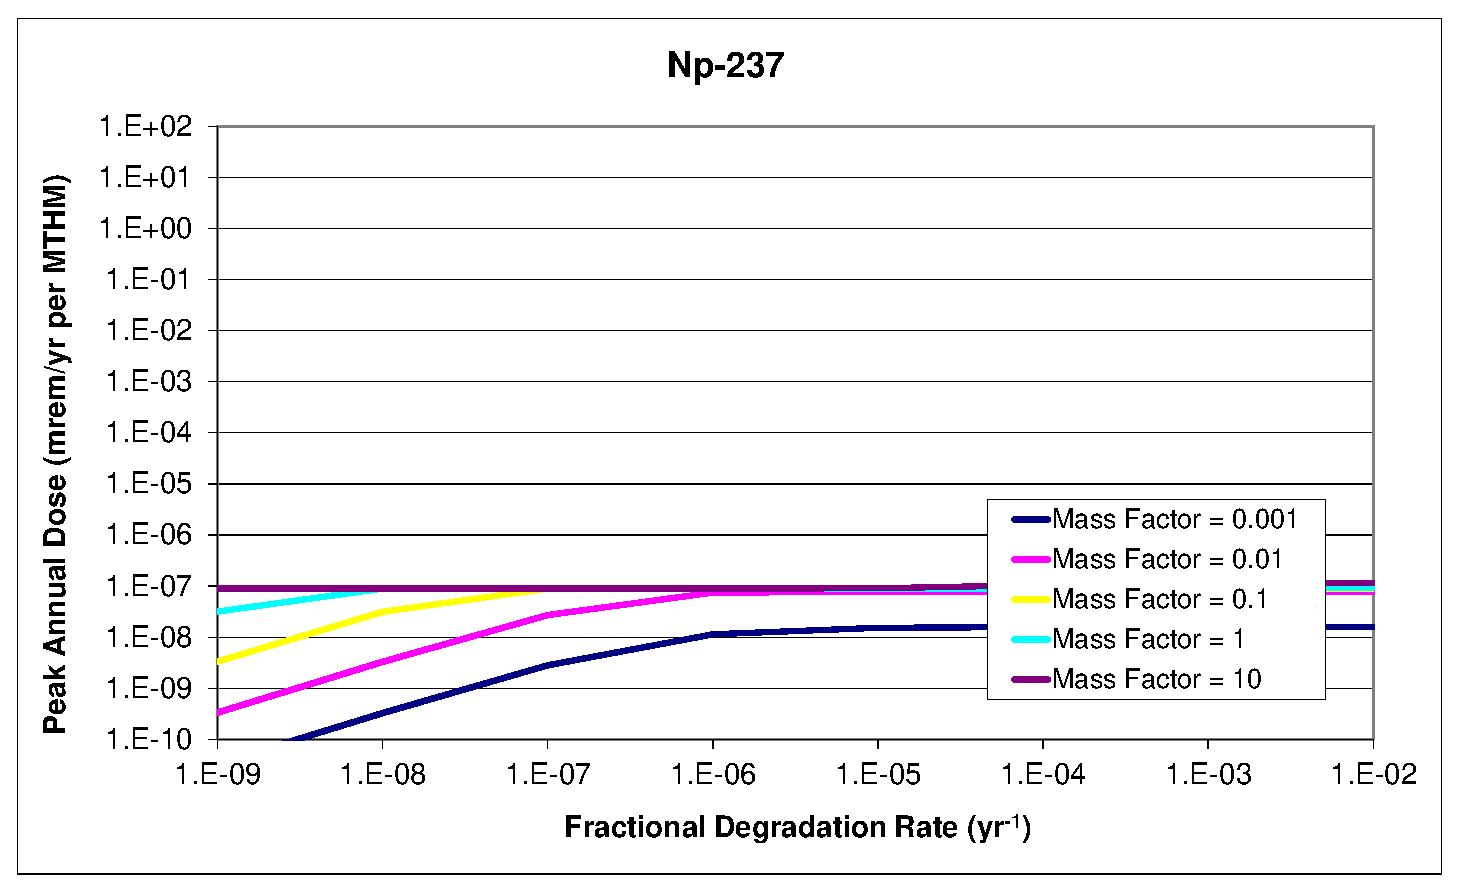
\includegraphics[width=\linewidth]{./chapters/nuclide_sensitivity/clay/AdvVelAndDiffCoeffEBSFail/Np-237.eps}
\caption{$^{237}Np$ reference diffusivity sensitivity.}
\label{fig:VAdvVelNp237}

\end{minipage}
\hspace{0.05\linewidth}
\begin{minipage}[b]{0.45\linewidth}

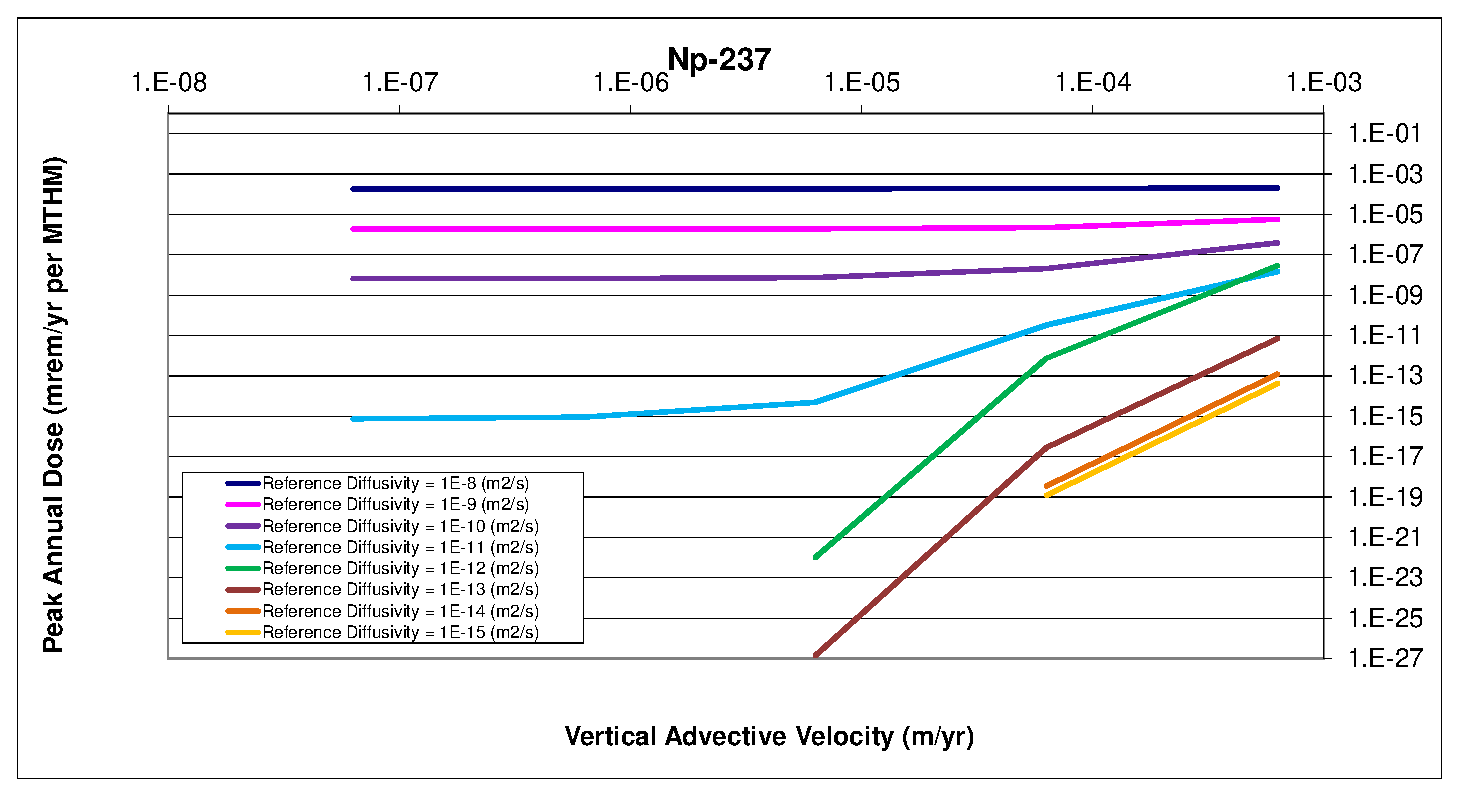
\includegraphics[width=\linewidth]{./chapters/nuclide_sensitivity/clay/AdvVelAndDiffCoeffEBSFail/Np-237-VAdvVel.eps}
\caption{$^{237}Np$ vertical advective velocity sensitivity.}
\label{fig:VAdvVelNp237VAdvVel}
  
\end{minipage}
\end{figure}

The convergence of the effect of the reference diffusivity and vertical 
advective velocity for the cases above shows the effect of dissolved 
concentration (solubility) limits and sorption. $Se$ is non-sorbing, but 
solubility limited.  The results from $^{79}Se$ in Figure \ref{fig:VAdvVelSe79} 
and \ref{fig:VAdvVelSe79VAdvVel} show that for low vertical advective velocity, 
the system is diffusion dominated.  However, for high vertical advective 
velocity, the diffusivity remains important even in the advective regime as 
spreading facilitates transport in the presence of solubility limited transport. 

\begin{figure}[htp!]
\begin{minipage}[b]{0.45\linewidth}
\centering
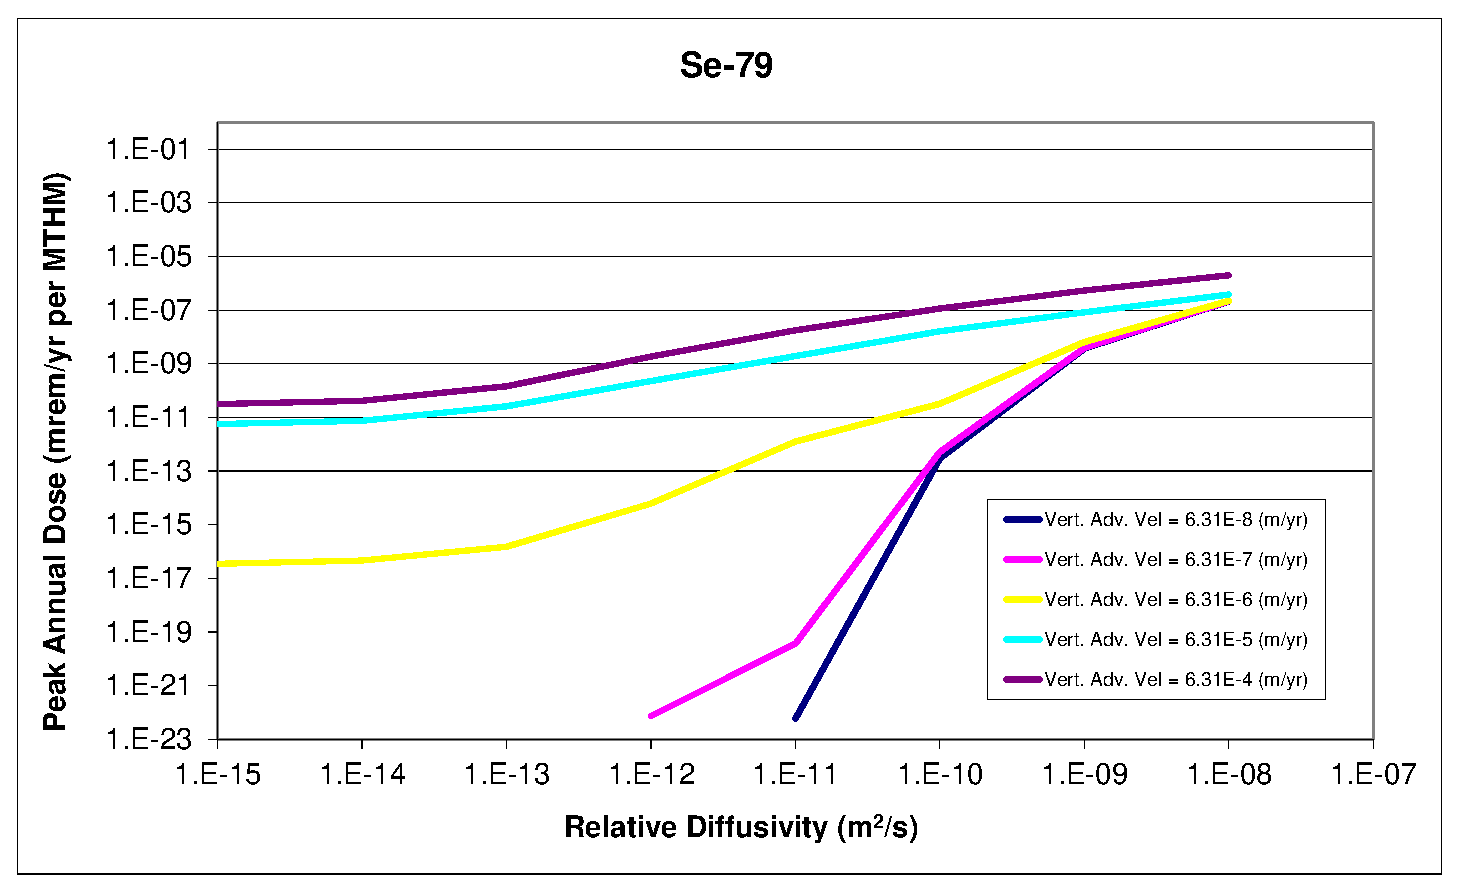
\includegraphics[width=\linewidth]{./chapters/nuclide_sensitivity/clay/AdvVelAndDiffCoeffEBSFail/Se-79.eps}
\caption{$^{79}Se$ reference diffusivity sensitivity.}
\label{fig:VAdvVelSe79}

\end{minipage}
\hspace{0.05\linewidth}
\begin{minipage}[b]{0.45\linewidth}

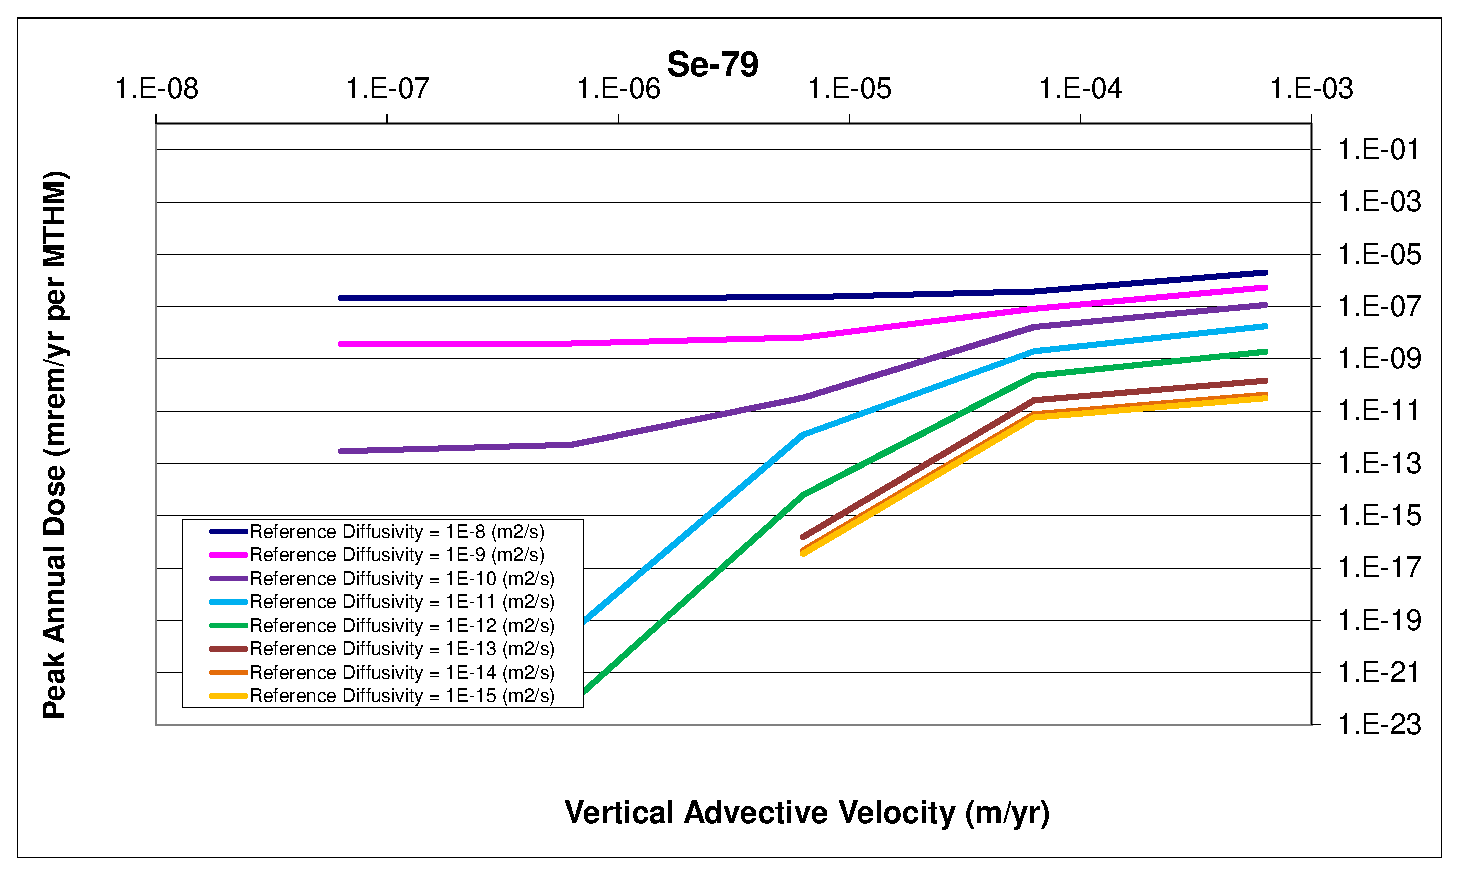
\includegraphics[width=\linewidth]{./chapters/nuclide_sensitivity/clay/AdvVelAndDiffCoeffEBSFail/Se-79-VAdvVel.eps}
\caption{$^{79}Se$ vertical advective velocity sensitivity.}
\label{fig:VAdvVelSe79VAdvVel}

\end{minipage}
\end{figure}
\FloatBarrier

\begin{frame}[ctb!]
\frametitle{Cyder Advective Diffusive Sensitivity}
\begin{figure}[ht]
\centering
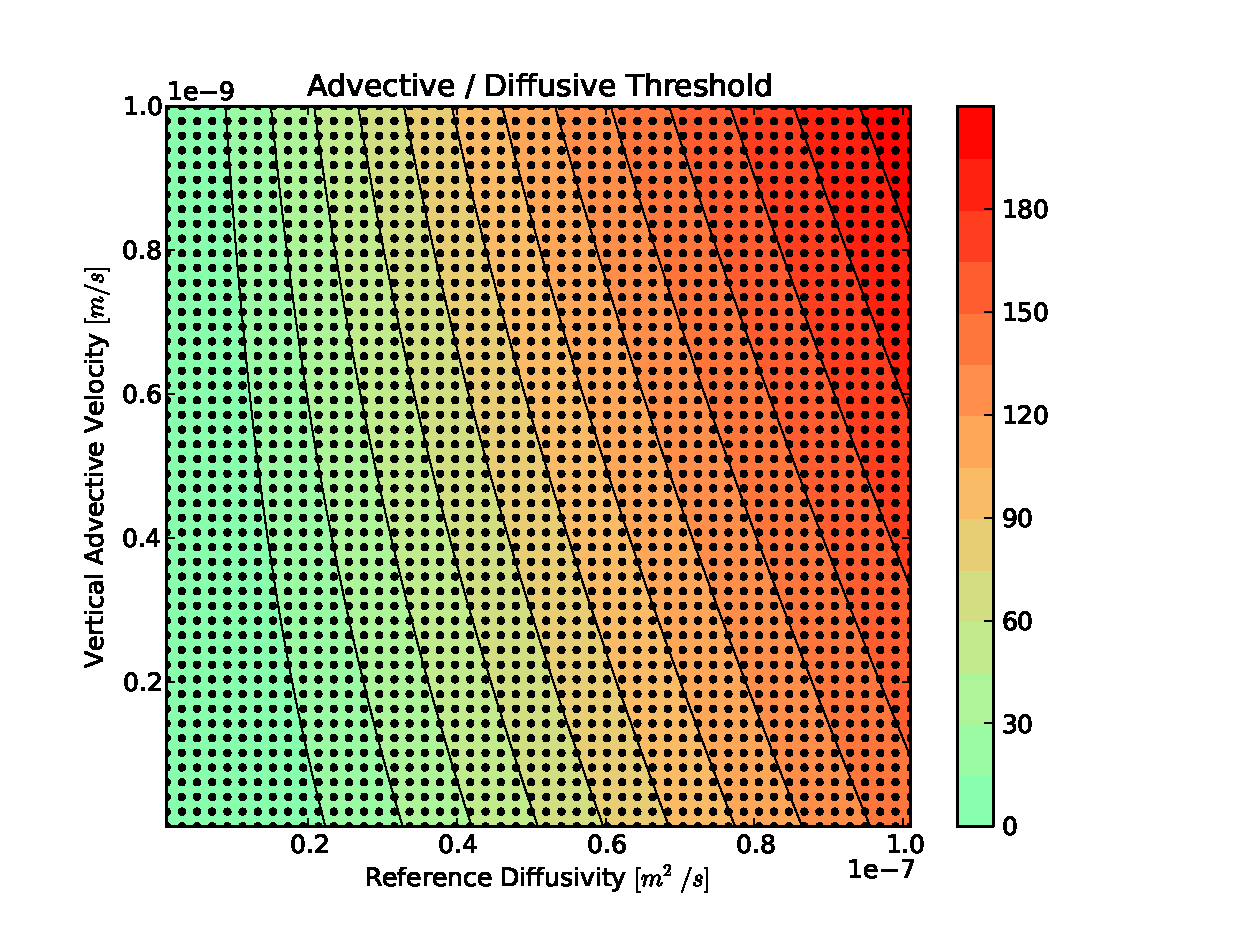
\includegraphics[height=0.7\textheight]{./nuclide_demonstration/adv_vel_diff.eps}
\caption[Advection vs. Diffusion Sensitivity in Cyder]{Dual advective velocity 
and reference diffusivity sensitivity for a non-sorbing, infinitely soluble 
nuclide. This demonstration utilized the Degradation Rate model and the coupled 
advective dispersive mass transfer mode.}
\label{fig:dr_adv_diff}
\end{figure}
\end{frame}


\section{LLNL Model Background}
% LLNL
\subsection{Analytical Model Background}
\begin{frame}[ctb!]
\frametitle{Analytical Model : Background}
The analytical  model
\begin{itemize} 
  \item was created at LLNL (H. Greenberg, J. Blink, et. al) \cite{hardin_generic_2011, sutton_investigations_2011, 
greenberg_application_2012}
  \item employs an analytic model from Carslaw and Jaeger \cite{carslaw_conduction_1959} 
  \item is implemented in MathCAD \cite{ptc_mathcad_2010}
  \item seeks to inform heat limited waste capacity calculations for 
    \begin{itemize}
      \item arbitrary geology 
      \item arbitrary waste package loading densities
      \item arbitrary homogeneous decay heat source
    \end{itemize}
\end{itemize}
\end{frame}

\begin{frame}
  \frametitle{Analytical Model : Geometry}
  \begin{figure}[h!]
    \begin{center}
      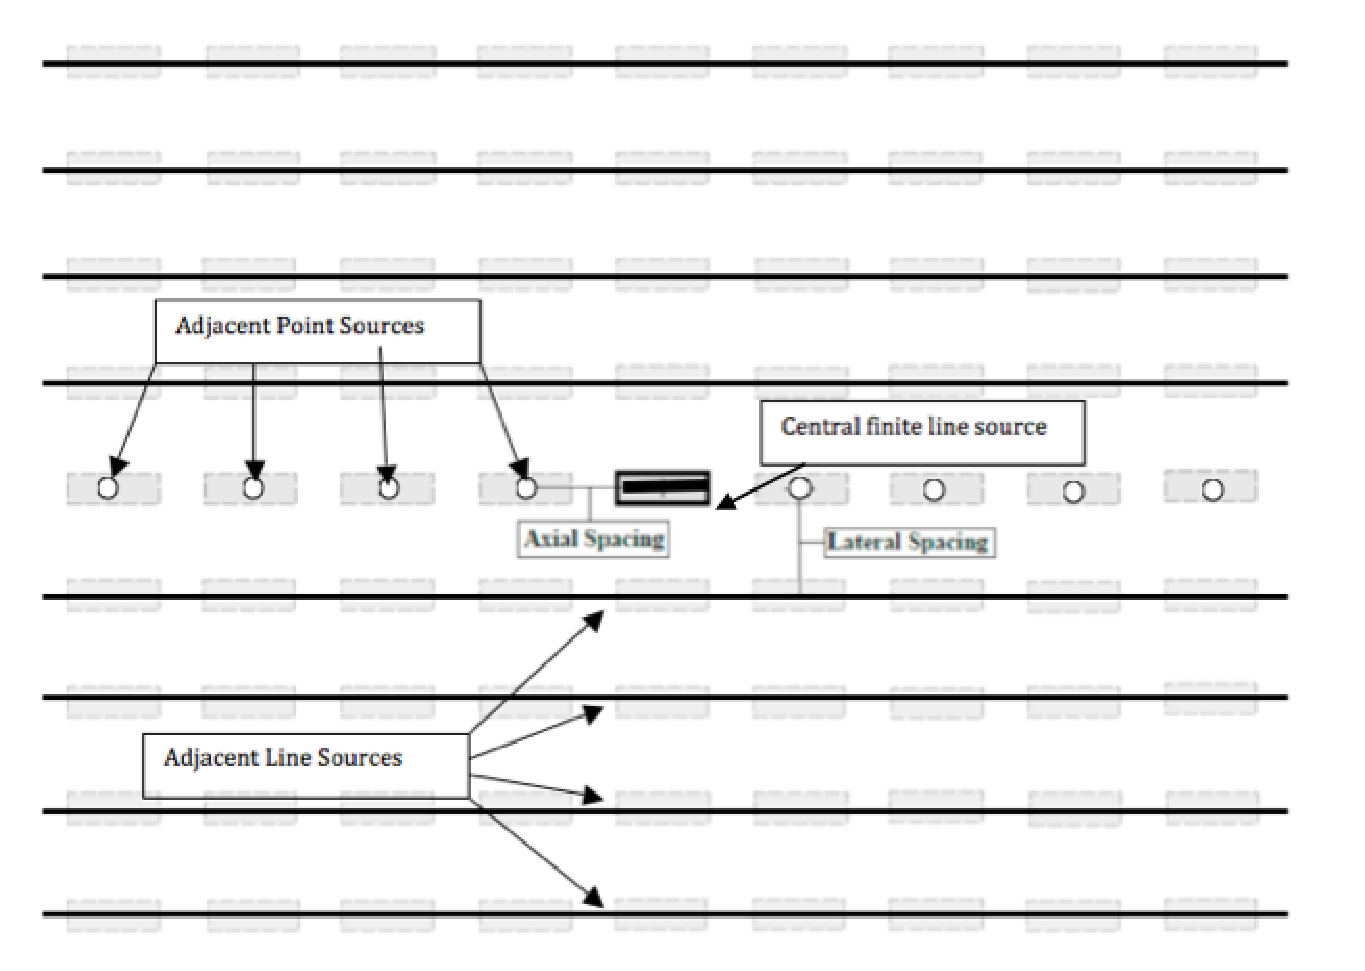
\includegraphics[width=0.7\textwidth]{./images/llnlConcept.eps}
    \caption{Vertical, horizontal, alcove, and borehole emplacement layouts can 
    be represented by a line of point sources and adjacent line sources 
    \cite{sutton_investigations_2011}.}
    \label{fig:llnl}
    \end{center}
  \end{figure}
\end{frame}

\begin{frame}
  \frametitle{Analytical Model : Calculation Method}
    LLNL's model is a MathCAD solution of the transient homogeneous 
    conduction equation,
    \begin{align}
      \nabla^2T  = \frac{1}{\alpha}\frac{\partial T}{\partial t},
      \label{condGl}
    \end{align}
    in which superimposed point and line source solutions approximate the repository 
    layout.
\end{frame}

\begin{frame}[ctb!]
\frametitle{Analytical Model : Calculation Method}
The model consists of two conceptual regions, an external region representing 
the host rock and an internal region representing the waste form, package, and 
buffer Engineered Barrier System within the disposal tunnel wall.   
\begin{itemize}
  \item Since the thermal mass of the EBS is small in comparison to the thermal 
    mass of the host rock, the internal region may be treated as quasi-steady 
    state.
  \item The transient state of the temperature at the calculation radius is 
    found with a convolution of the transient external solution with the steady 
    state internal solution.
  \item The internal and external regions are \textbf{approximated} to be a 
    single homogeneous medium.
  \item The process is then iterated with a one year resolution in order to 
    arrive at a temperature evolution over the lifetime of the repository. 
\end{itemize}
\end{frame}


\begin{frame}[ctb!]
\frametitle{Analytical Model : Calculation Method}
\begin{minipage}{0.3\textwidth}
\begin{figure}[h!]
  \begin{center}
    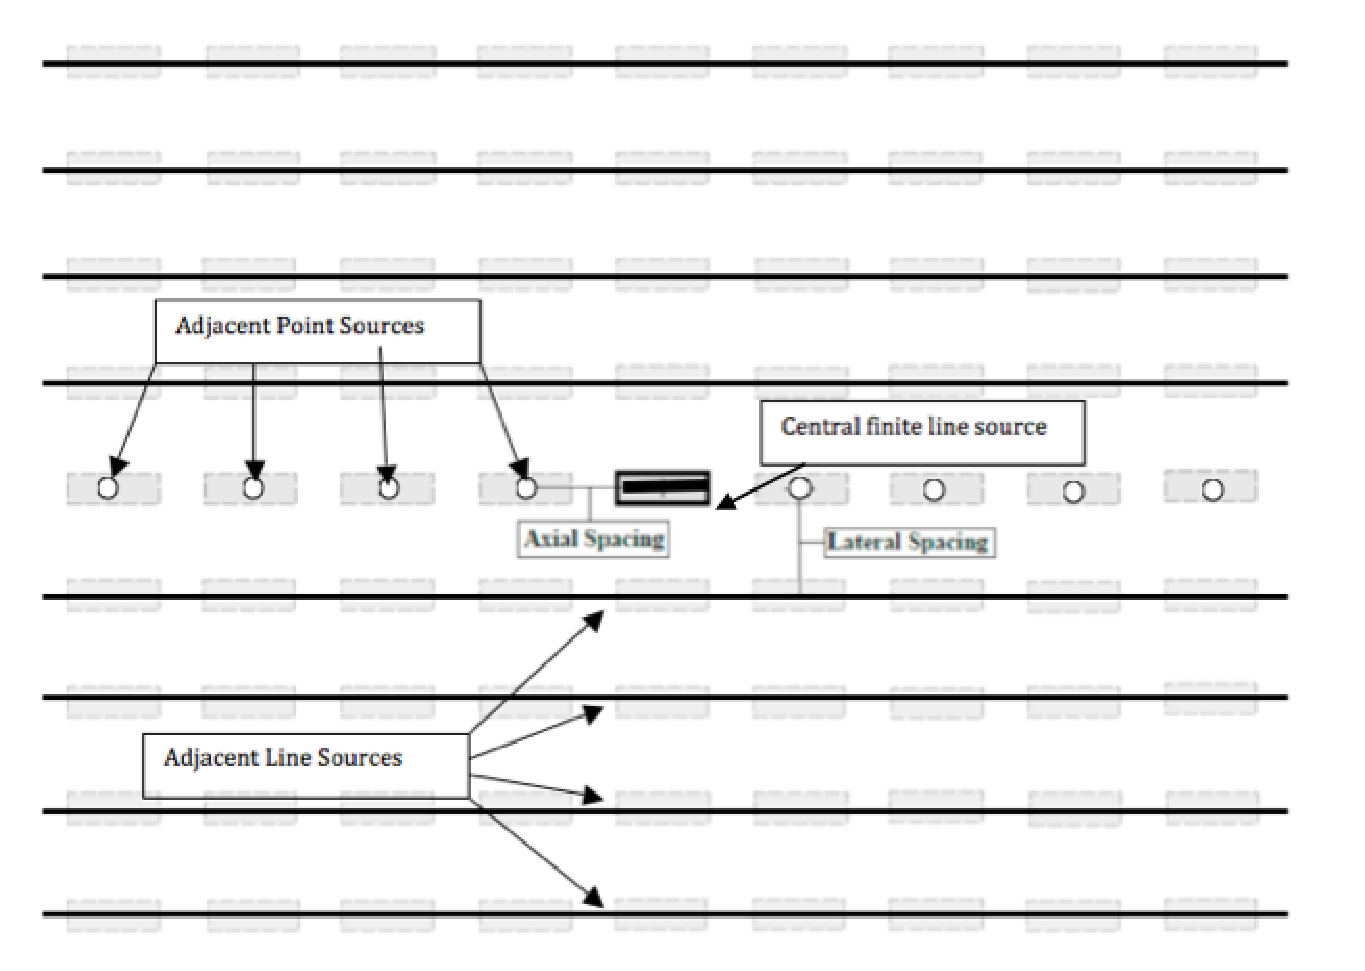
\includegraphics[width=\textwidth]{./images/llnlConcept.eps}
  \end{center}
  \caption{The central package is represented by a finite line source
  \cite{sutton_investigations_2011}.}
  \label{fig:llnl}
\end{figure}
\end{minipage}
\hspace{0.01mm}
\begin{minipage}{0.6\textwidth}
The geometric layout of the analytic LLNL model in Figure \ref{fig:llnl} 
shows  that the central package is represented by the finite line solution
\footnotesize{
\begin{align}
  T_{line}&(t,x,y,z) = \nonumber\\
  &\frac{1}{8\pi K_{th}} 
  \bigintsss_0^t\!\frac{q_L(t')}{t-t'}e^{ \frac{-\left(x^2 + z^2\right)}{4\alpha 
  (t-t')} }\nonumber\\ &\cdot\left[ \erf{\left[ \frac{1}{2} \frac{\left( y + 
  \frac{L}{2} \right)}{\sqrt{\alpha(t-t')}}  \right]} - \erf{\left[ \frac{1}{2} 
  \frac{\left( y - \frac{L}{2} \right)}{\sqrt{\alpha(t-t')}}  \right]} 
  \right]\,\mathrm{dt'}.
  \label{line}
\end{align}
}
\end{minipage}
\end{frame}

\begin{frame}[ctb!]
\frametitle{Analytical Model : Calculation Method}
\begin{minipage}{0.3\textwidth}
\begin{figure}[h!]
  \begin{center}
    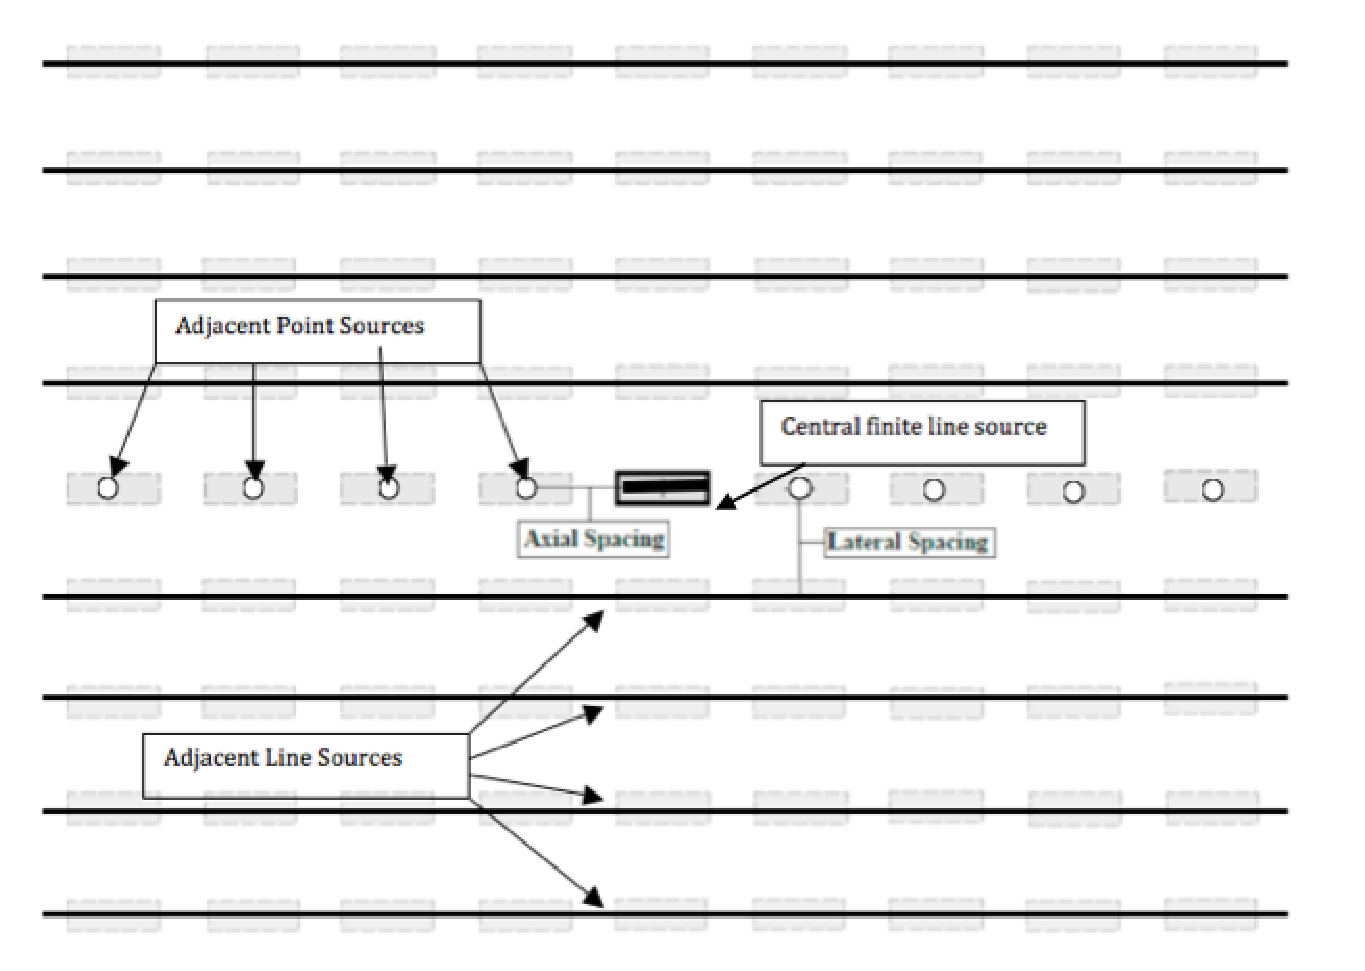
\includegraphics[width=\textwidth]{./images/llnlConcept.eps}
  \end{center}
  \caption{Adjacent packages are represented as point sources
  \cite{sutton_investigations_2011}.}
  \label{fig:llnl}
\end{figure}
\end{minipage}
\hspace{0.1mm}
\begin{minipage}{0.6\textwidth}
 Adjacent packages within the central tunnel are represented by the point source 
 solution,
 \footnotesize{
  \begin{align}
    T_{point}(t,r) &= \frac{1}{8K_{th}\sqrt{\alpha}\pi^{\frac{3}{2}}}\nonumber\\
     &\bigintsss_0^{t}\!\frac{q(t')}{(t-t')^{\frac{3}{2}}}e^{\frac{-r^2}{4\alpha(t-t')}}\,\mathrm{dt'}.
    \label{point}
  \end{align}
  }
  \end{minipage}
\end{frame}


\begin{frame}[ctb!]
\frametitle{Analytical Model : Calculation Method}
\begin{minipage}{0.3\textwidth}
\begin{figure}[h!]
  \begin{center}
    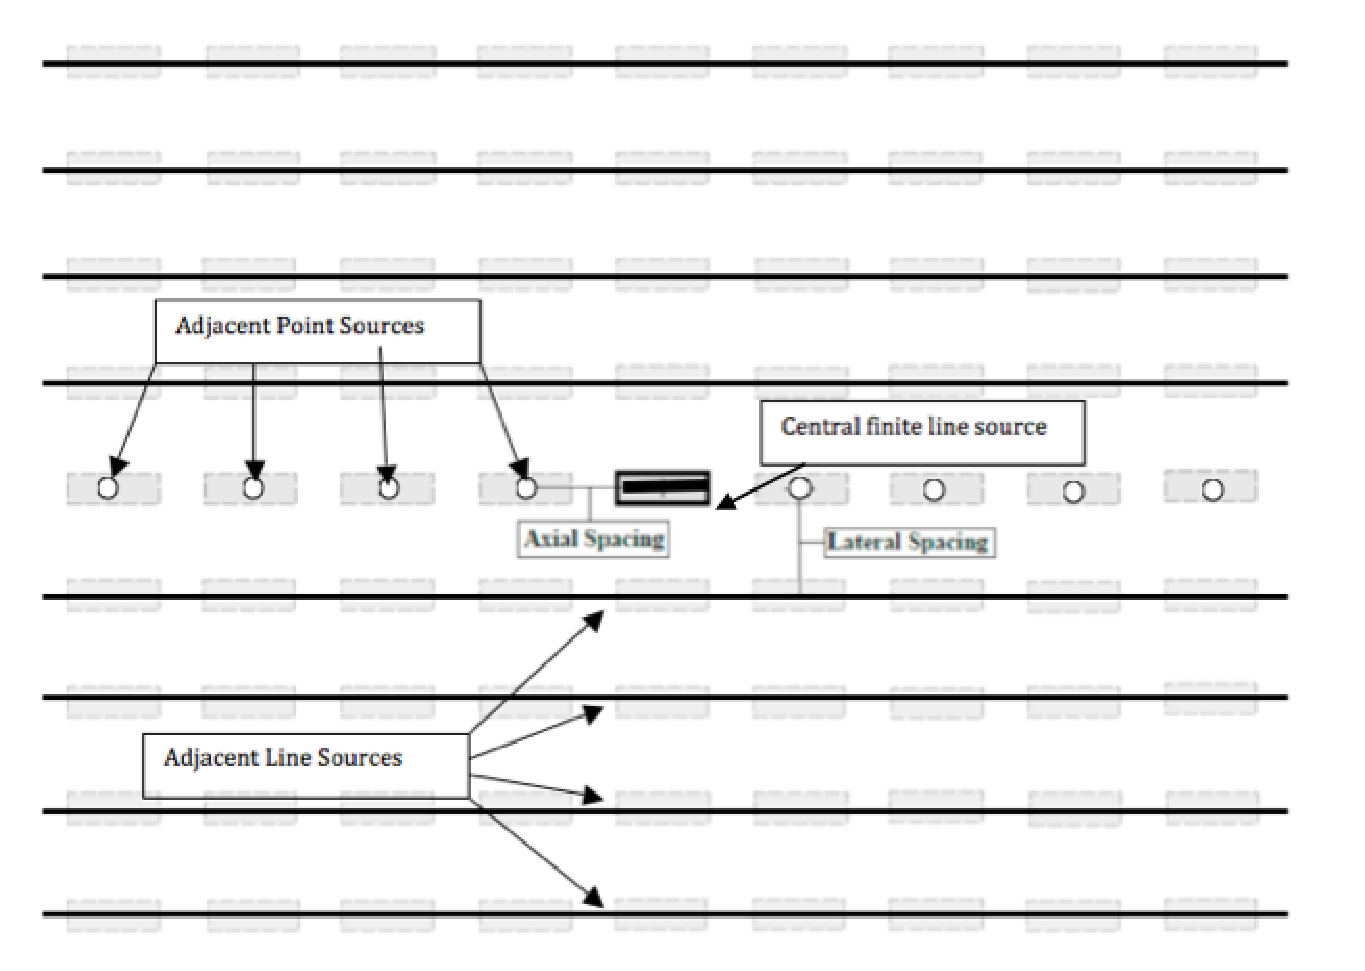
\includegraphics[width=\textwidth]{./images/llnlConcept.eps}
  \end{center}
  \caption{The non-central disposal tunnels are represented as infinite line sources
  \cite{sutton_investigations_2011}.}
  \label{fig:llnl}
\end{figure}
\end{minipage}
\hspace{0.1mm}
\begin{minipage}{0.6\textwidth}
Adjacent disposal tunnels are represented by the infinite line source solution,
\footnotesize{
\begin{align}
  T_{\infty line}(t,x,z) &= \frac{1}{4\pi K_{th}} 
  \bigintsss_0^t\frac{q_L(t')}{t-t'}e^{ \frac{-\left(x^2 + z^2\right)}{4\alpha 
  (t-t')} }
  \label{infline}
  \intertext{in infinite homogeneous media, where}
  \alpha &= ~~\mbox{thermal diffusivity } [m^2\cdot s^{-1}]\nonumber\\
  q(t) &= ~~\mbox{point heat source} [W]\nonumber\\
  \intertext{and}
  q_L(t) &= ~~\mbox{linear heat source} [W\cdot m^{-1}]\nonumber
\end{align}
}
Superimposed point and line source solutions allow for a notion of the 
repository layout to be modeled in the host rock.
\end{minipage}
\end{frame}



\section{Geologic Media and Concepts}
\begin{frame}[ctb!]
  \frametitle{Clay Disposal Environments}
  \footnotesize{

  \begin{figure}[h!]
    \begin{center}
      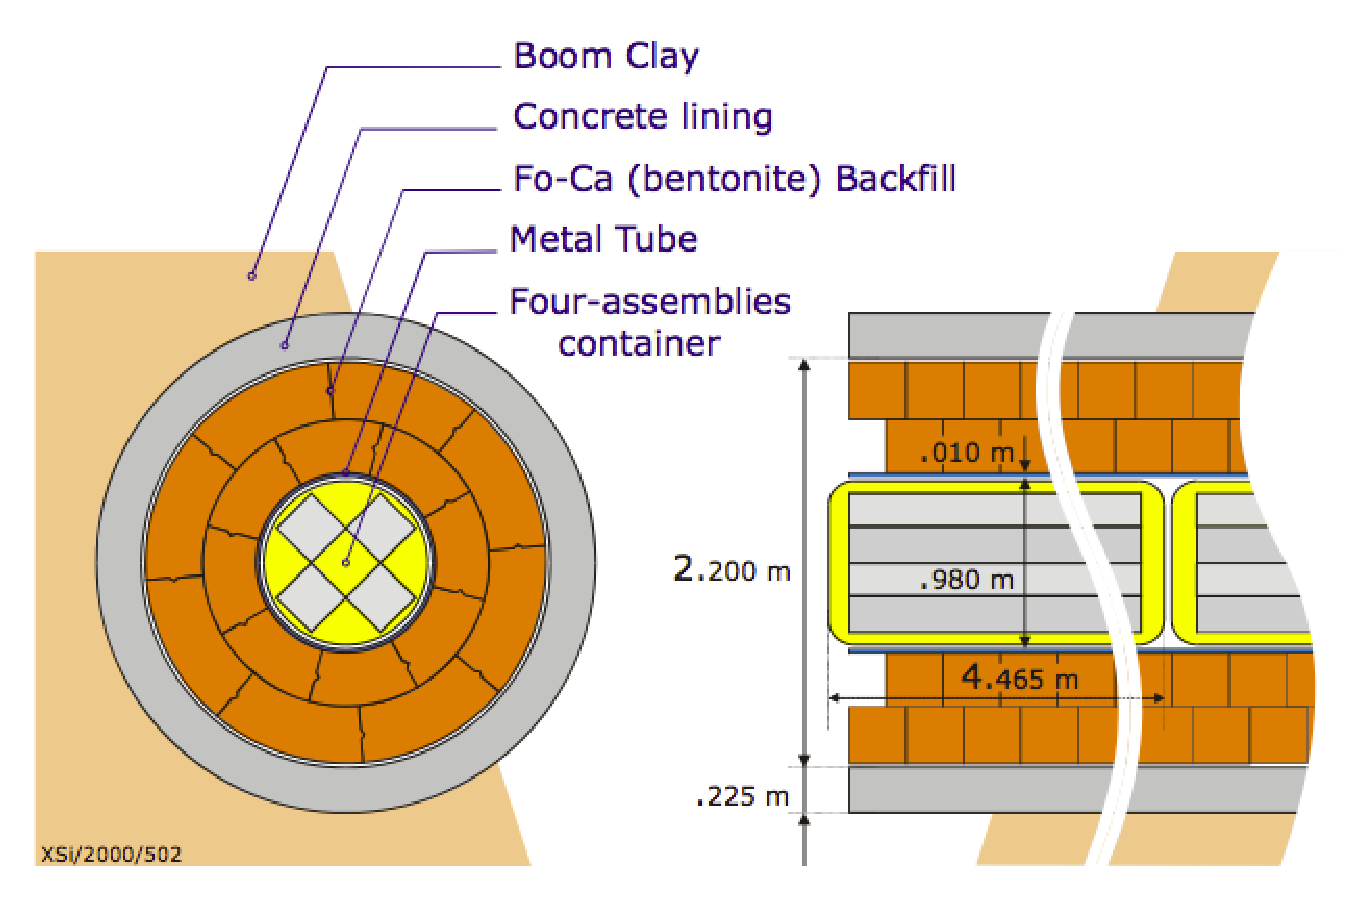
\includegraphics[height=.7\textheight]{./images/belgianClayRedImp.eps}
    \end{center}
    \caption{Belgian reference concept in Boom Clay 
    \cite{von_lensa_red-impact_2008}.}
    \label{fig:belgianClayRedImp}
  \end{figure}

}
\end{frame}

\begin{frame}[ctb!]
  \frametitle{Granite Disposal Environments}
  \footnotesize{

  \begin{figure}[h!]
    \begin{center}
      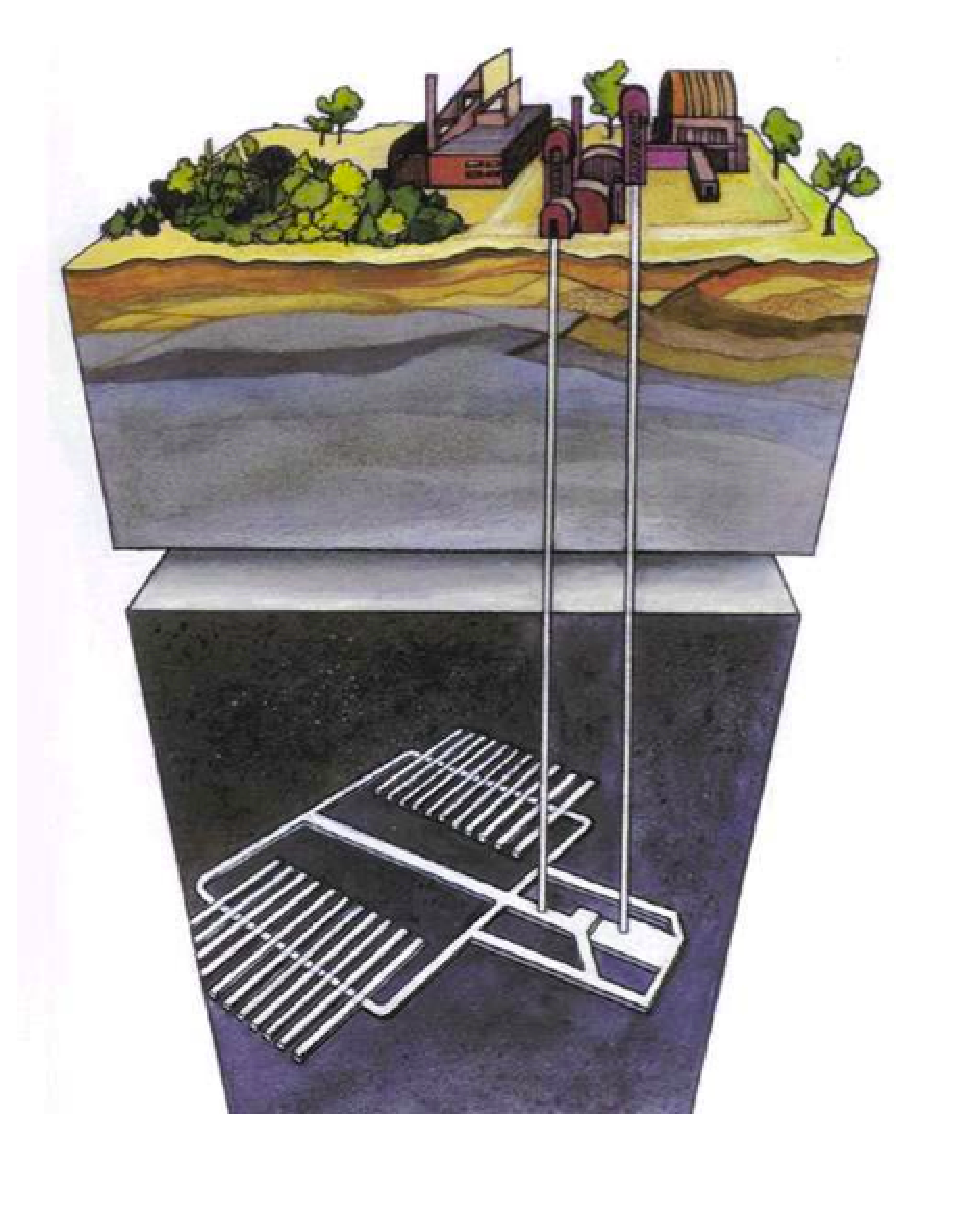
\includegraphics[height=.7\textheight]{./images/czechGraniteRedImp.eps}
    \end{center}
    \caption{Czech reference concept in Granite 
    \cite{von_lensa_red-impact_2008}.}
    \label{fig:czechGraniteRedImp}
  \end{figure}
}
\end{frame}

\begin{frame}[ctb!]
  \frametitle{Salt Disposal Environments}
  \footnotesize{

  \begin{figure}[h!]
    \begin{center}
      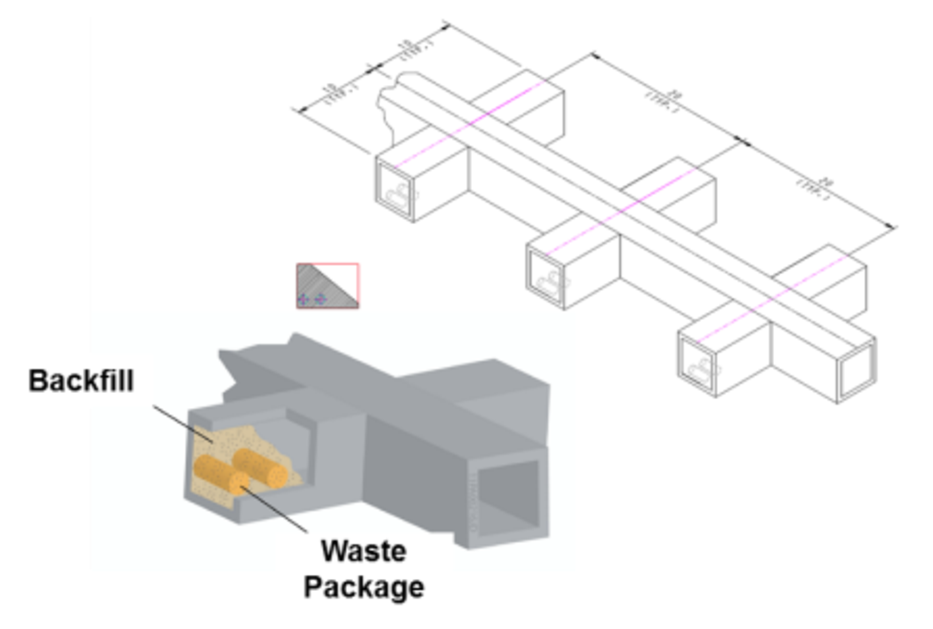
\includegraphics[height=.7\textheight]{./images/carter_salt_layout.eps}
    \end{center}
    \caption{DOE-NE Used Fuel Disposition Campaign  concept in 
    Salt \cite{hardin_generic_2011}.}
    \label{fig:salt_layout}
  \end{figure}
}
\end{frame}
\begin{frame}[ctb!]
  \frametitle{Salt Disposal Environments}
  \footnotesize{

  \begin{figure}[h!]
    \begin{center}
      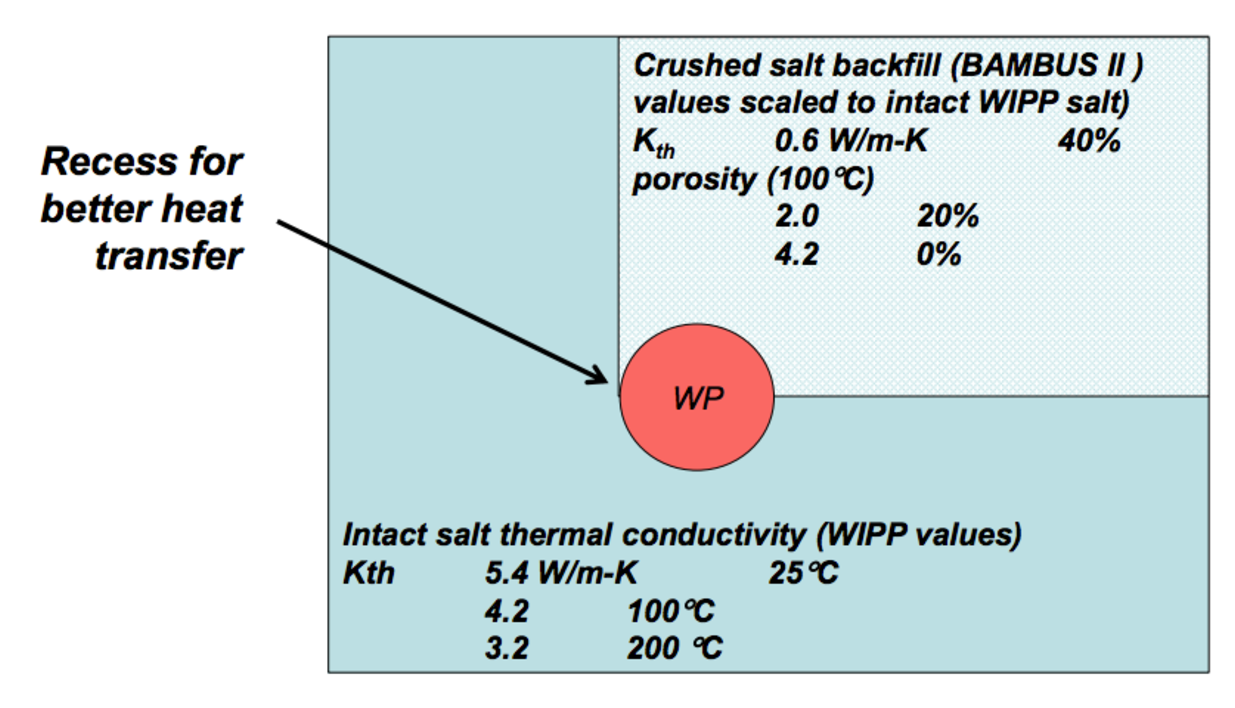
\includegraphics[height=.7\textheight]{./images/hardin_salt_layout.eps}
    \end{center}
    \caption{DOE-NE Used Fuel Disposition Campaign  concept in 
    Salt \cite{hardin_generic_2011}.}
    \label{fig:hardin_salt_layout}
  \end{figure}
}
\end{frame}

\begin{frame}[ctb!]
  \frametitle{Deep Borehole Disposal Environment}
  \footnotesize{

  \begin{figure}[h!]
    \begin{center}
      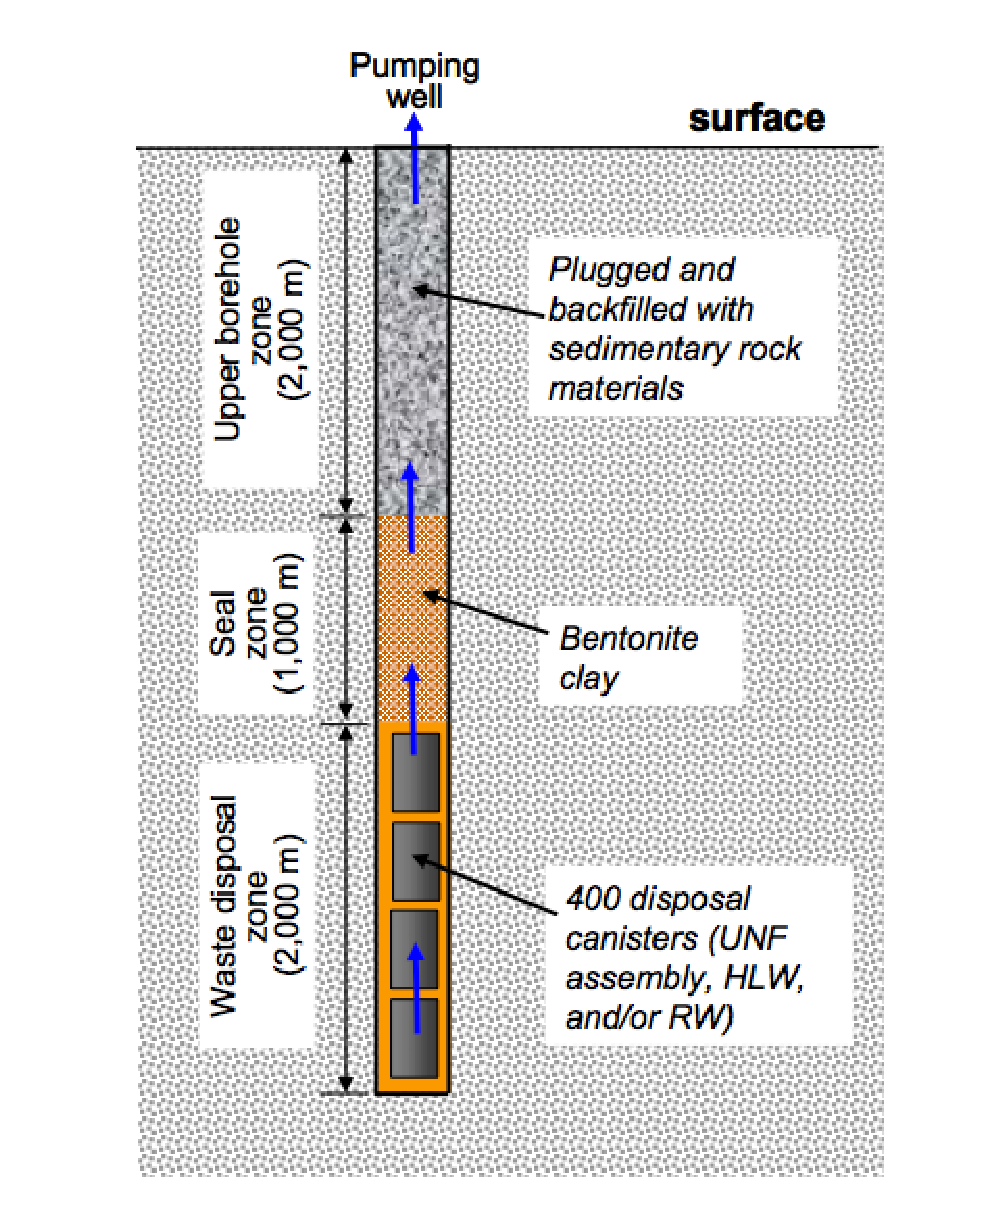
\includegraphics[height=.7\textheight]{./images/boreholeGPAM.eps}
    \end{center}
    \caption{DOE-NE Used Fuel Disposition Campaign Deep Borehole concept 
    \cite{hardin_generic_2011}.}
    \label{fig:boreholeGPAM}
  \end{figure}
}
\end{frame}

%%----------------------------------------%%
\begin{frame}[ctb!]
  \frametitle{Engineered Barriers : Waste Forms}
\footnotesize{
  The first line of defense is the waste form.
  \begin{figure}[htbp!]
  \begin{center}
    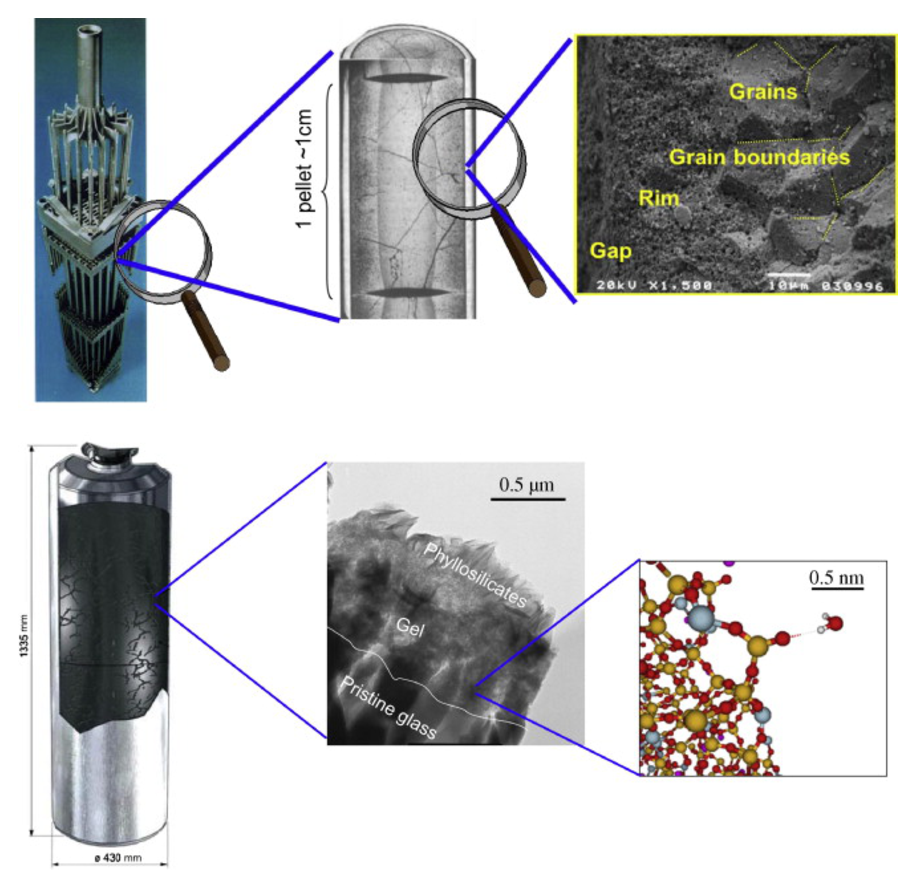
\includegraphics[width=0.5\textwidth]{./images/waste_forms_poinssot.eps}
  \end{center}
  \caption{A comparison of uranium oxide and borosilicate glass waste forms 
  \cite{poinssot_long-term_2012}.}
  \label{fig:waste_forms_poinssot}
\end{figure}

}
\end{frame}

%%----------------------------------------%%
\begin{frame}[ctb!]
  \frametitle{Engineered Barriers : Waste Packages}
\footnotesize{
  \begin{figure}[htbp!]
  \begin{center}
    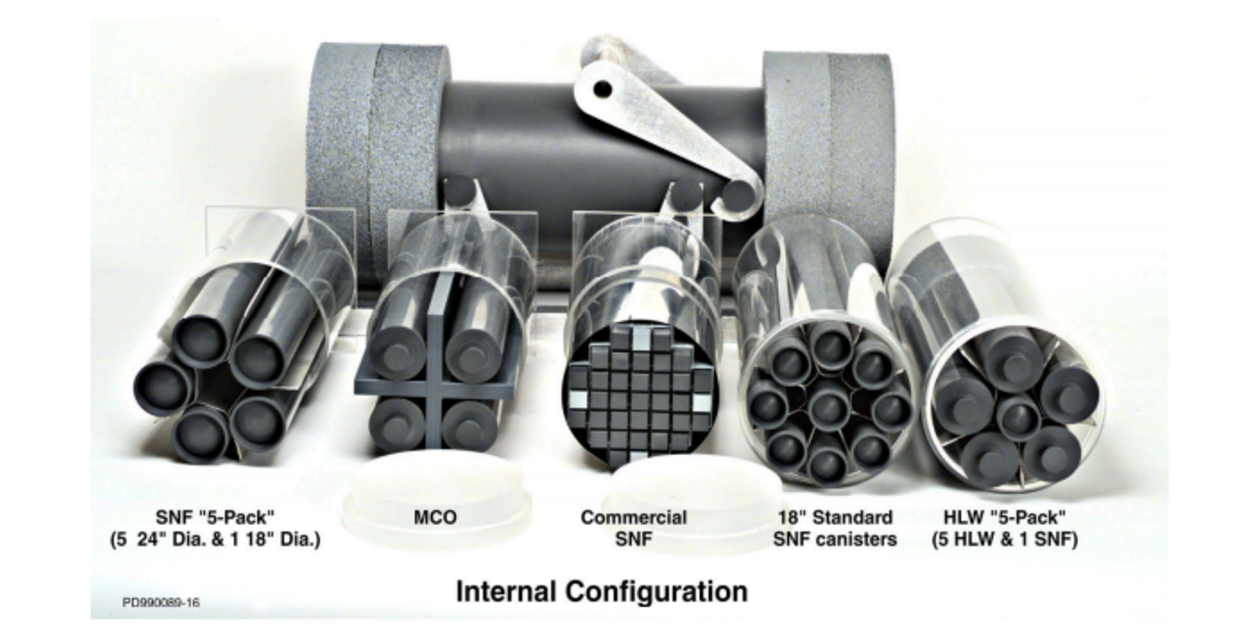
\includegraphics[width=0.7\textwidth]{./images/packages_ineel.eps}
  \end{center}
  \caption{Conceptual mockup of waste packages around waste forms 
    \cite{bridges_standardized_2001}.}
  \label{fig:packages}
\end{figure}

}
\end{frame}

%%----------------------------------------%%
\begin{frame}[ctb!]
  \frametitle{Engineered Barriers : Disposal Cask}
\footnotesize{
  \begin{figure}[htbp!]
  \begin{center}
    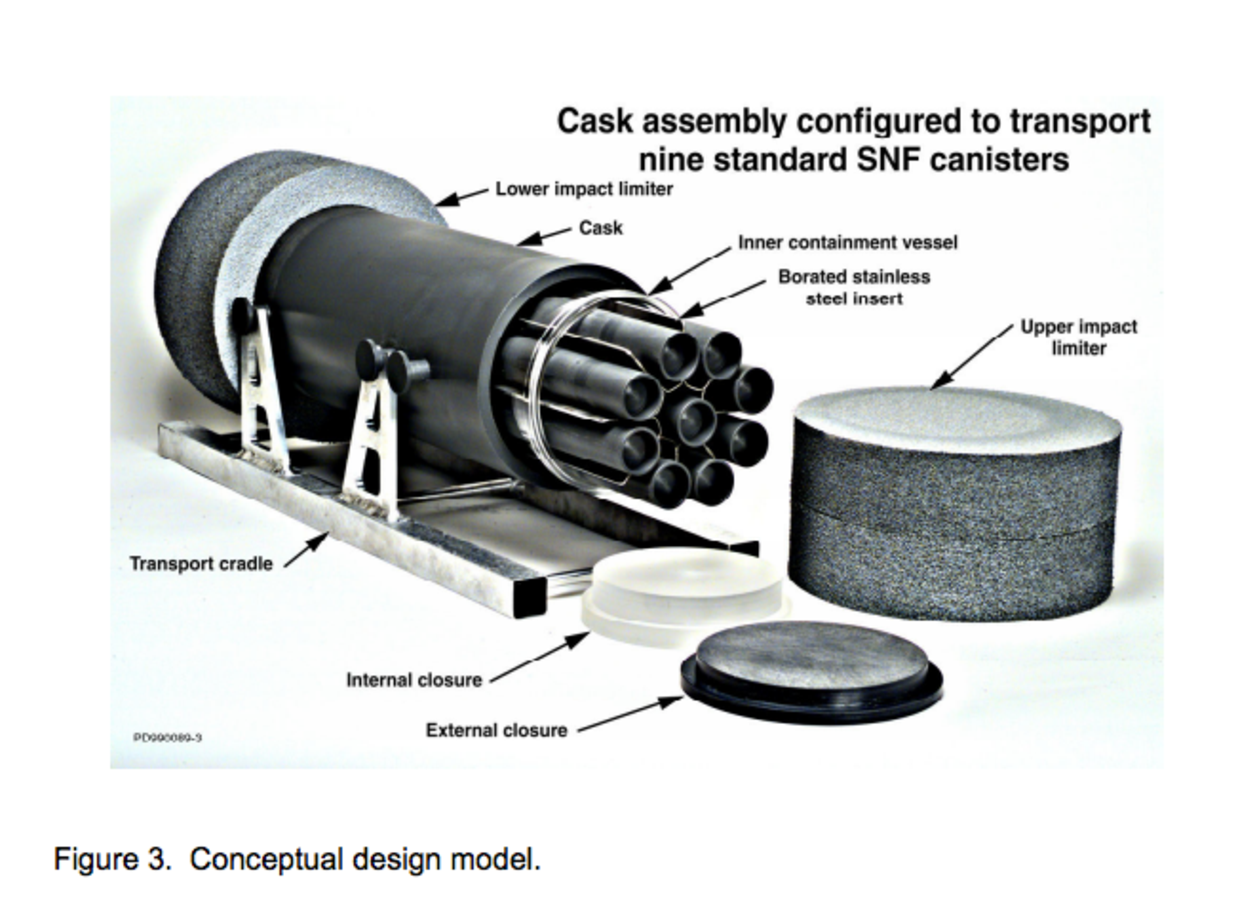
\includegraphics[width=0.7\textwidth]{./images/cask_ineel.eps}
  \end{center}
  \caption{Conceptual mockup of a transport and disposal cask 
    \cite{bridges_standardized_2001}.}
  \label{fig:packages}
\end{figure}

}
\end{frame}

%%----------------------------------------%%
\begin{frame}[ctb!]
  \frametitle{Engineered Barriers : Buffer}
\footnotesize{
  \begin{figure}[h!]
    \begin{center}
      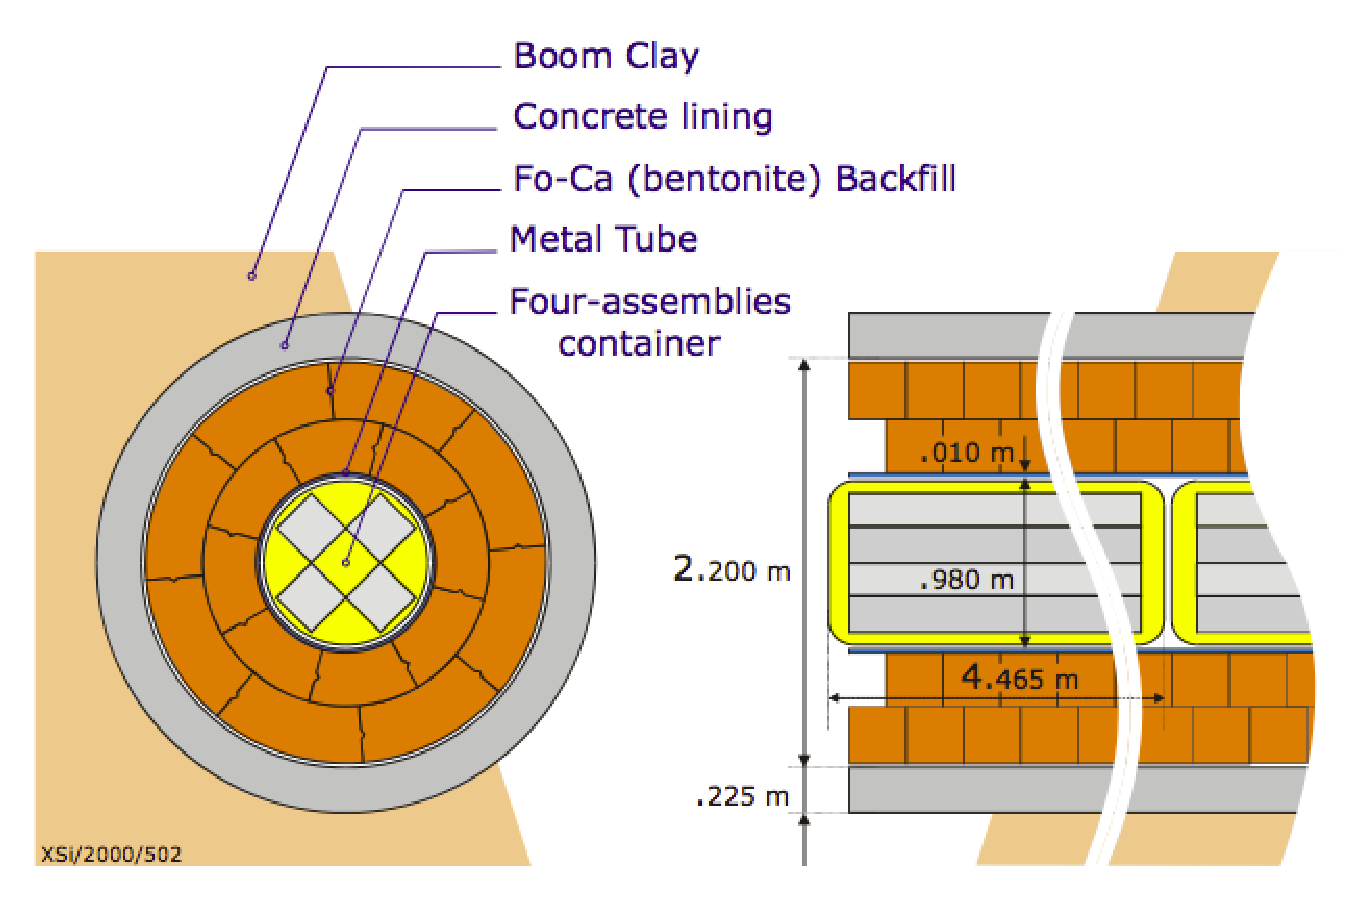
\includegraphics[height=.7\textheight]{./images/belgianClayRedImp.eps}
    \end{center}
    \caption{Belgian reference concept in Boom Clay 
    \cite{von_lensa_red-impact_2008}.}
    \label{fig:belgianClayRedImp}
  \end{figure}
}
\end{frame}

%%----------------------------------------%%
\begin{frame}[ctb!]
  \frametitle{Natural Barrier : Geology}
\footnotesize{
  \begin{figure}[htbp!]
  \begin{center}
    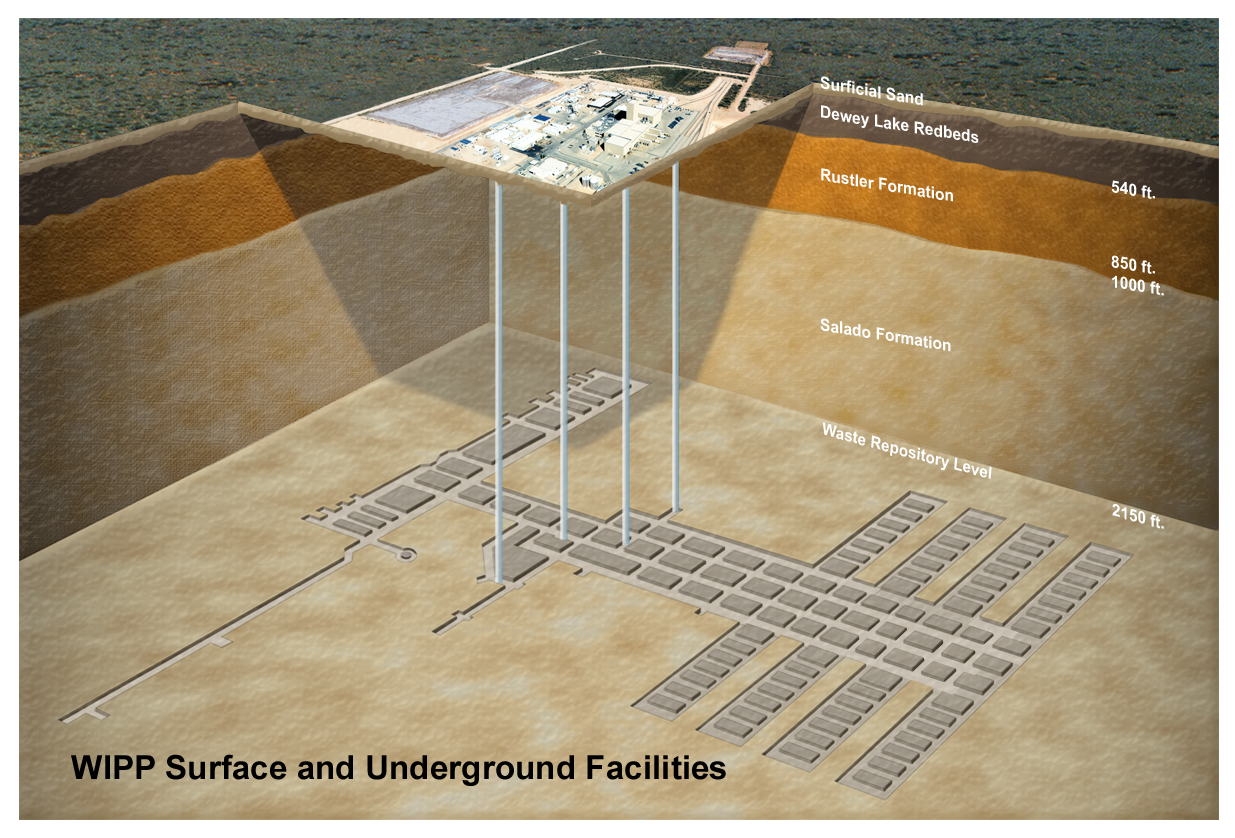
\includegraphics[width=0.7\textwidth]{./images/wipp_stratigraph.eps}
  \end{center}
  \caption{The Waste Isolation Pilot Plant has many geologic layers above the 
    salt bed \cite{doe_wipp_2013}.}
  \label{fig:wipp}
\end{figure}

}
\end{frame}
\begin{frame}
  \frametitle{Repository Layouts}

  \begin{minipage}{0.49\textwidth}
    \begin{figure}[h!]
      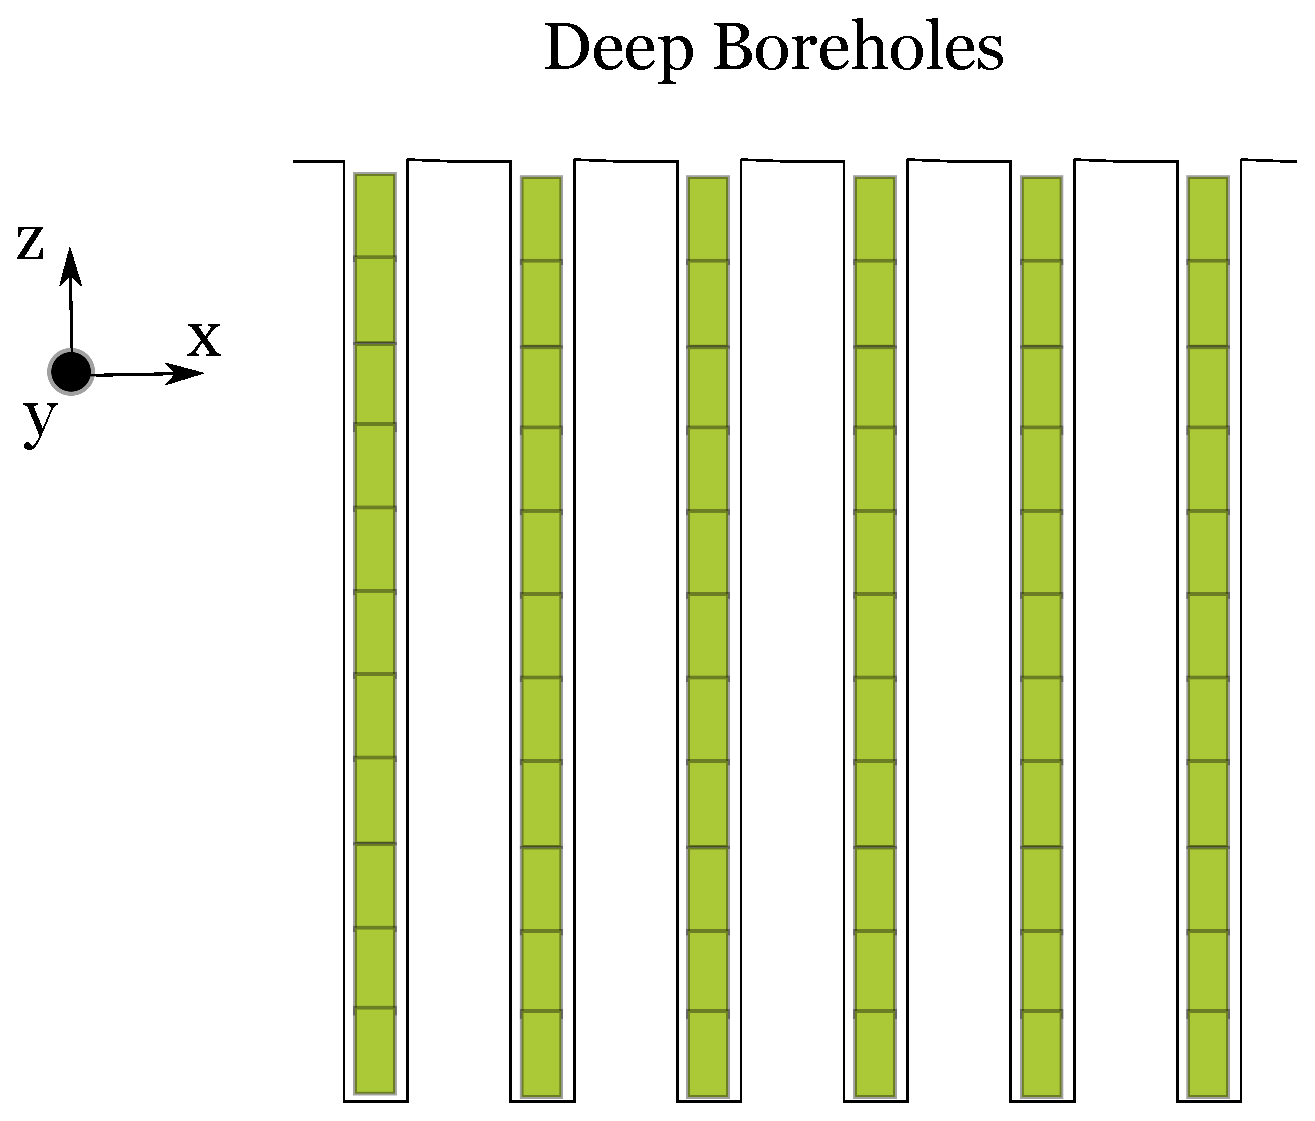
\includegraphics[width=0.75\textwidth]{./images/boreholes.eps}
    \end{figure}
    \begin{figure}[h!]
      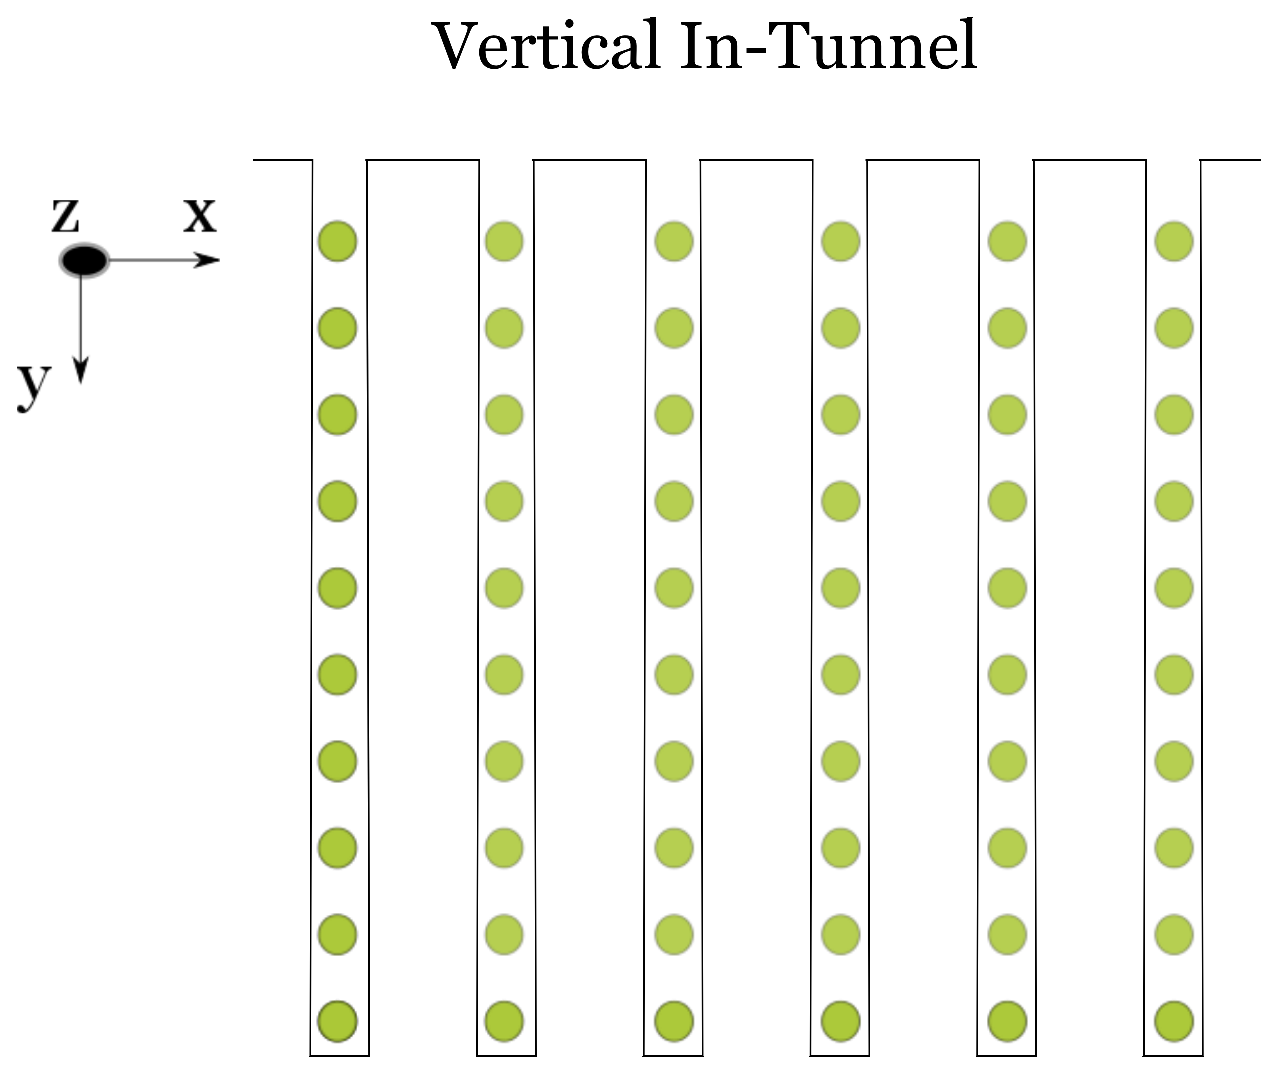
\includegraphics[width=0.75\textwidth]{./images/vertical.eps}
    \end{figure}
  \end{minipage}
  \hspace{0.01cm}
  \begin{minipage}{0.49\textwidth}
    \begin{figure}[h!]
      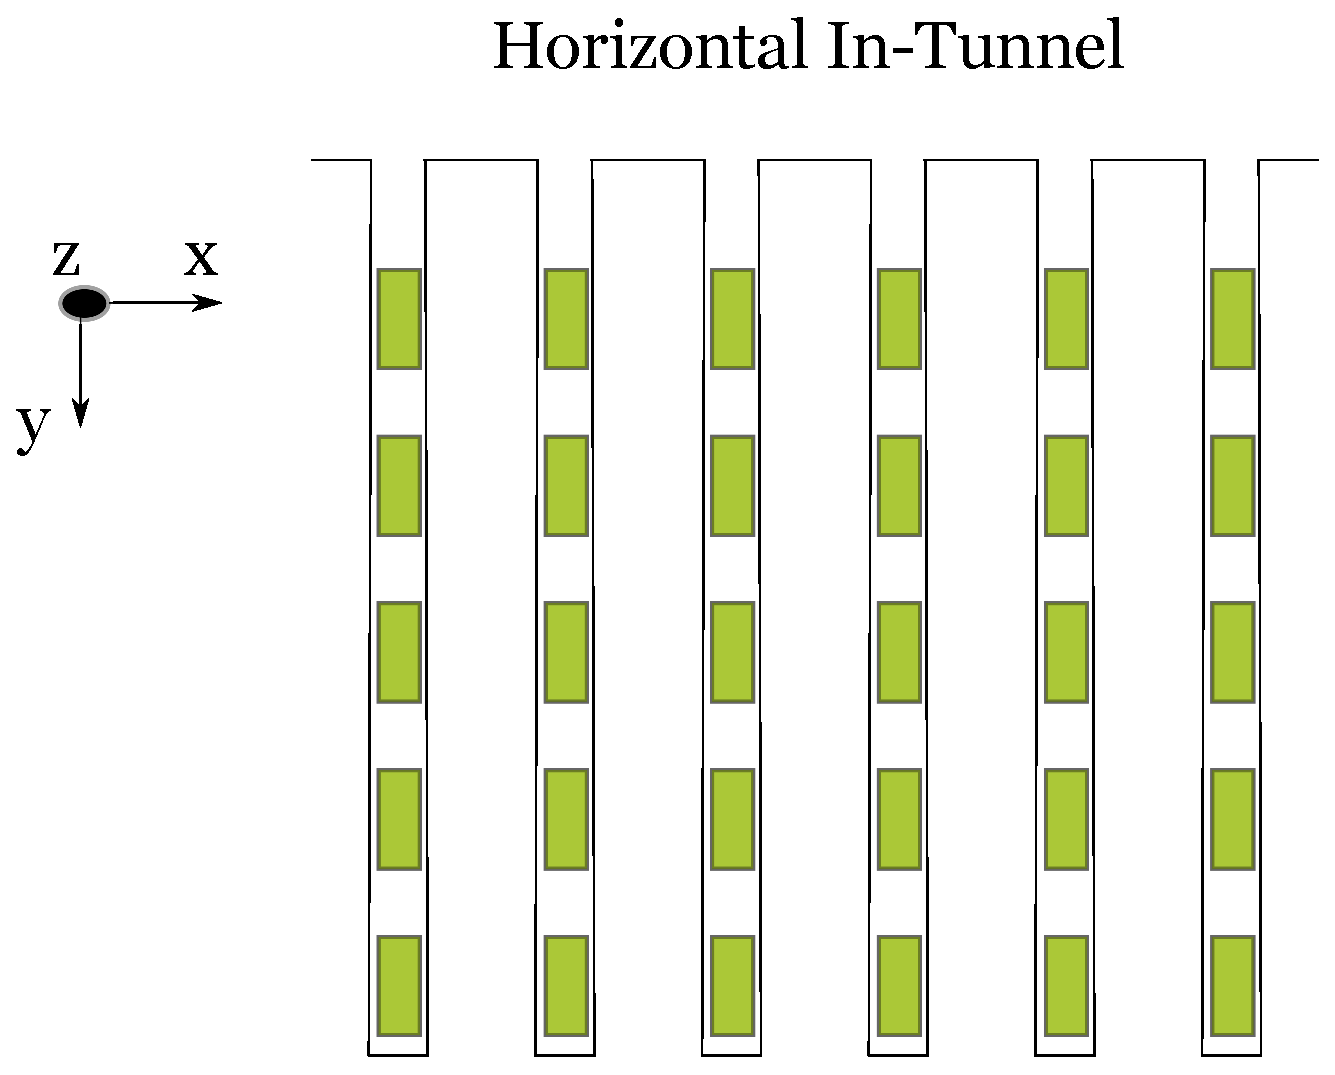
\includegraphics[width=0.8\textwidth]{./images/horizontal.eps}
    \end{figure}
    \begin{figure}[h!]
      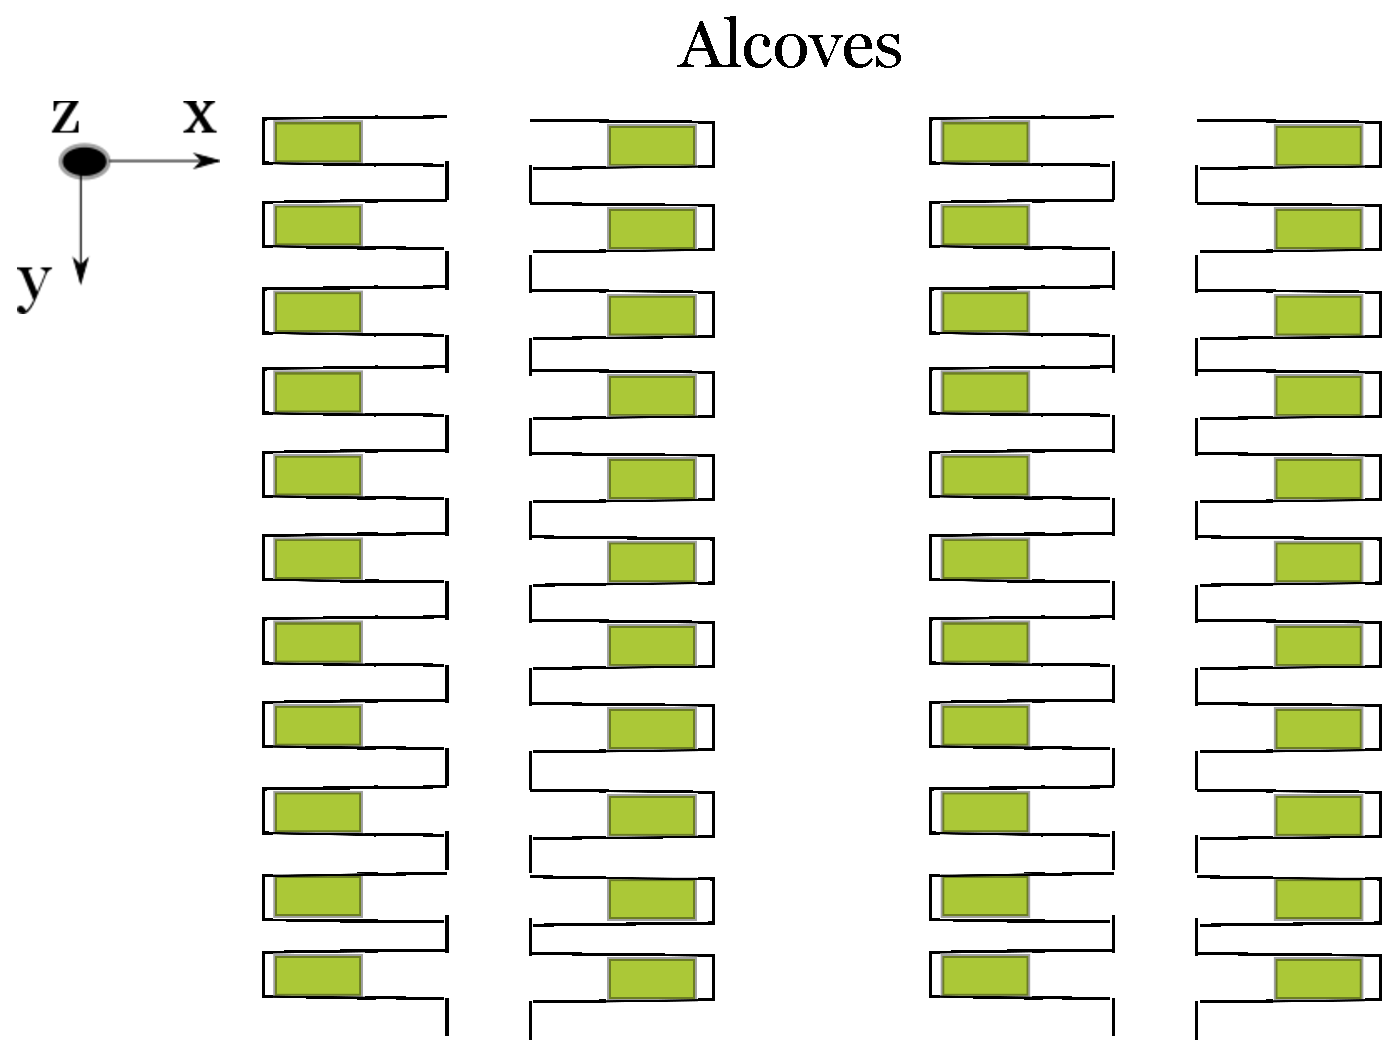
\includegraphics[width=0.8\textwidth]{./images/alcoves.eps}
    \end{figure}
  \end{minipage}

\end{frame}

\begin{frame}[ctb!]
  \footnotesize{
  \frametitle{Unsaturated, Ventilated Concepts}
  \begin{figure}[htbp!]
  \begin{center}
    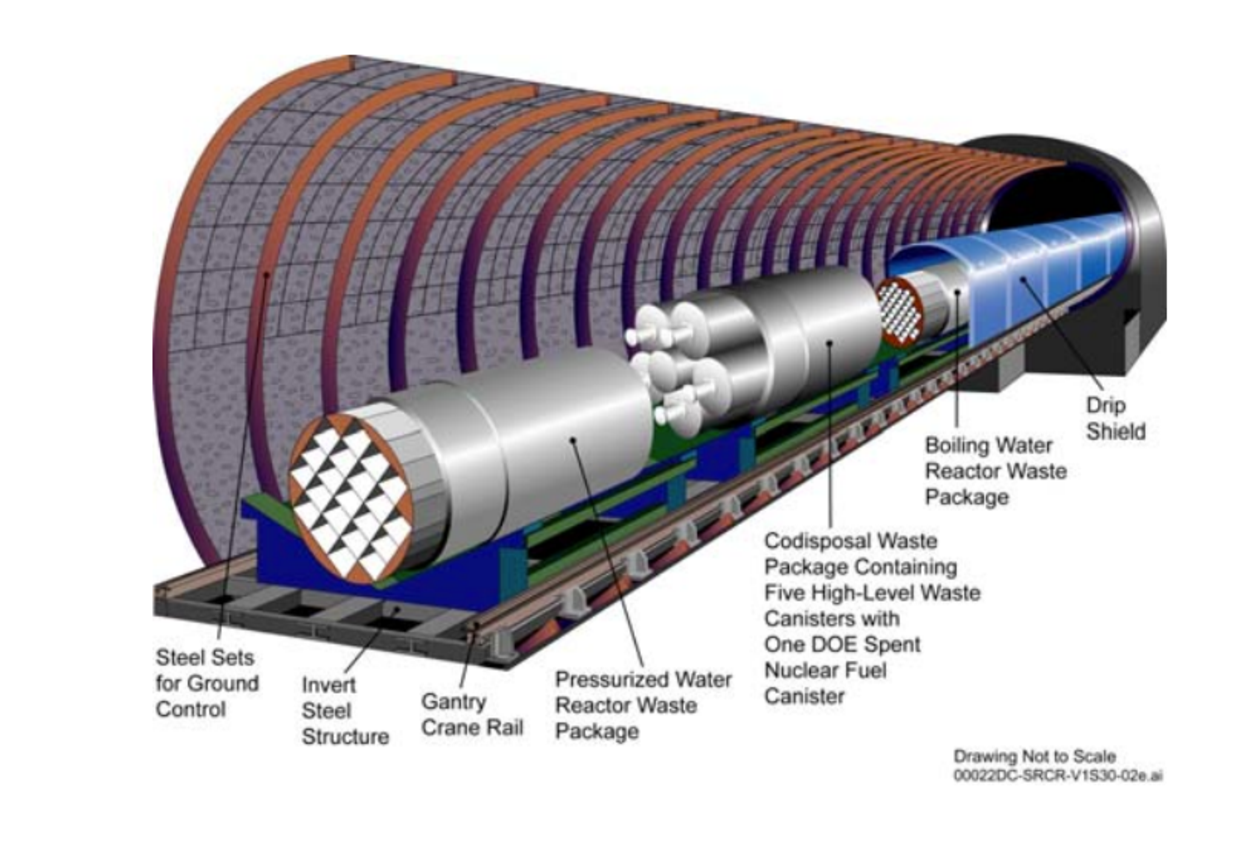
\includegraphics[height=0.7\textwidth]{./images/yucca_tunnel.eps}
  \end{center}
  \caption{The current U.S. geologic disposal concept \cite{peters_whats_2013}.}
  \label{fig:yucca_tunnel}
\end{figure}

}
\end{frame}

\begin{frame}[ctb!]
  \footnotesize{
  \frametitle{Saturated , Enclosed Concepts} 
 \begin{figure}[h!]
    \begin{center}
      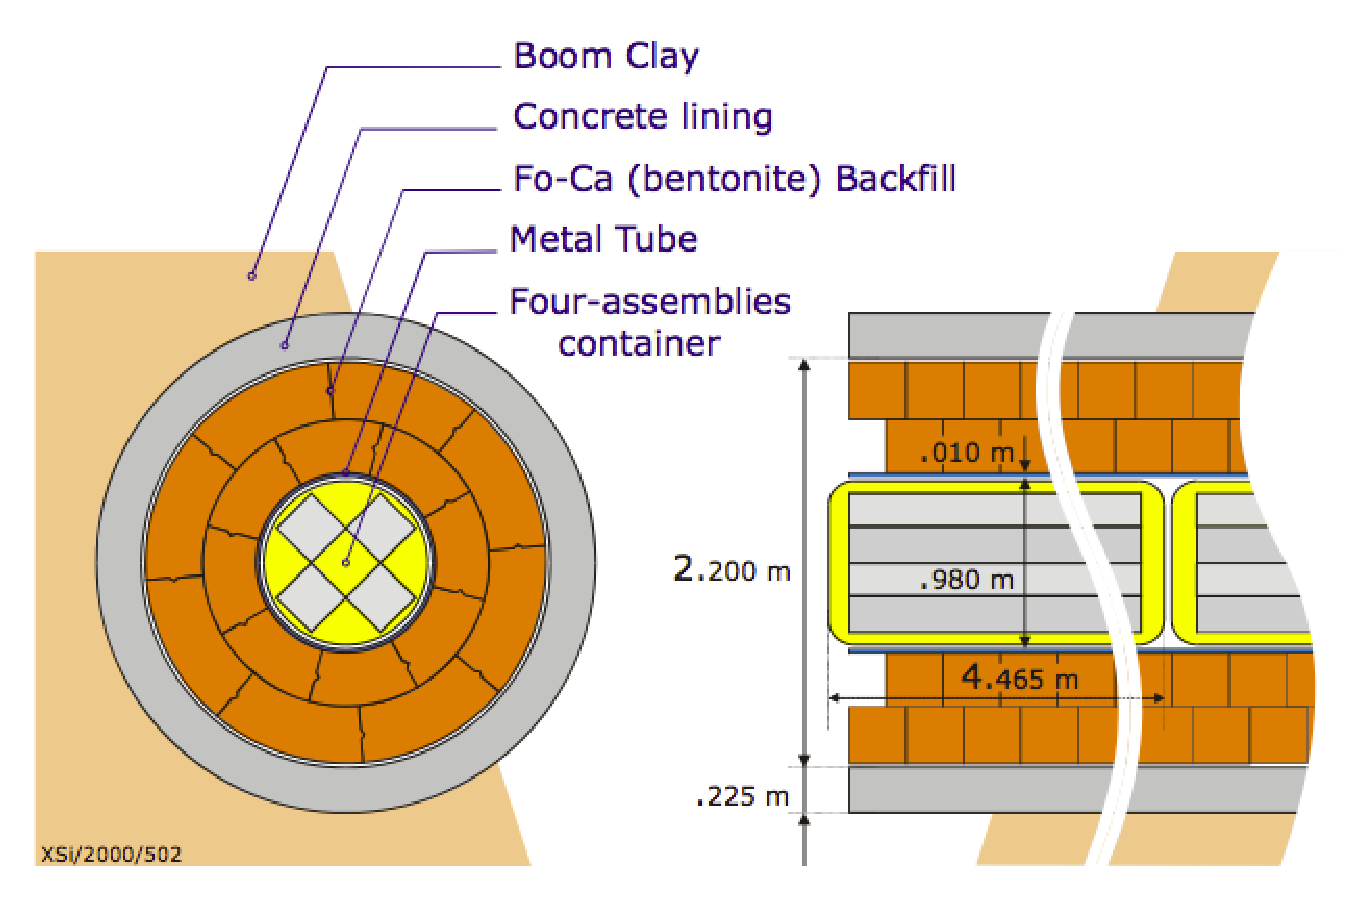
\includegraphics[height=.7\textheight]{./images/belgianClayRedImp.eps}
    \end{center}
    \caption{The Belgian reference concept in Boom Clay is backfilled very soon
   after waste emplacement without a ventilation period and is located below the water table
   \cite{von_lensa_red-impact_2008}.}
    \label{fig:belgianClayRedImp}
  \end{figure}
}
\end{frame}

\setcounter{framenumber}{\value{finalframe}}
\section{Mixed Cell Model}

\begin{frame}
  \frametitle{Radionuclide Transport : Mixed Cell Sorption}
  \footnotesize{

The mass of contaminant sorbed into the degraded and precipitated solids can be
found using a linear isotherm model \cite{schwartz_fundamentals_2004},
characterized by the relationship 
\begin{align}
s_{i} &= K_{di} c_{i}
\label{linear_iso}
\intertext{where}
s_i &= \mbox{ the solid concentration of isotope i }[kg/kg]\nonumber\\
K_{di} &= \mbox{ the distribution coefficient of isotope i}[m^3/kg]\nonumber\\
c_i &= \mbox{ the liquid concentration of isotope i }[kg/m^3].\nonumber
\end{align}

  From the sorbed contaminant mass, we find the non-sorbed contaminant mass in the free fluid,

\begin{align}
m_{ffl}   &= m_{ffT} - \frac{1}{2} \left(m_{ffT} - m_{psm} - \frac{V_{ff}}{K_d}\right) \nonumber\\
          & \mp \frac{1}{2} \sqrt{m_{ffT}^2 + 2m_{ffT}\left(m_{psm} - 
          \frac{V_{ff}}{K_d}\right) + \left(m_{psm} + 
          \frac{V_{ff}}{K_d}\right)^2}.
\label{m_ffl_full}
\intertext{where}
m_{ffT}  &= \mbox{ total degraded contaminant mass }[kg]\nonumber\\
m_{psm}  &= \mbox{ noncontaminant mass in degraded and precipitated solids }[kg]\nonumber\\
m_{psc}  &= \mbox{ contaminant mass in degraded and precipitated solids }[kg]\nonumber\\
\rho_b   &= \mbox{ bulk (dry) density of the medium }[kg/m^3].\nonumber\\
\end{align}

    }
\end{frame}
